\documentclass[12pt]{article}
\usepackage[pdfborder={0 0 0.5 [3 2]}, plainpages=false]{hyperref}%
\usepackage[left=1in,right=1in,top=1in,bottom=1in]{geometry}%
\usepackage[shortalphabetic]{amsrefs}%
\usepackage{amsmath}
\usepackage{enumerate}
% \usepackage{enumitem}
\usepackage{amssymb}                
\usepackage{amsmath}                
\usepackage{amsfonts}
\usepackage{amsthm}
\usepackage{bbm}
\usepackage[table,xcdraw]{xcolor}
\usepackage{tikz}
\usepackage{float}
\usepackage{booktabs}
\usepackage{svg}
\usepackage{mathtools}
\usepackage{cool}
\usepackage{url}
\usepackage{graphicx,epsfig}
\usepackage{makecell}
\usepackage{array}

\def\noi{\noindent}
\def\T{{\mathbb T}}
\def\R{{\mathbb R}}
\def\N{{\mathbb N}}
\def\C{{\mathbb C}}
\def\Z{{\mathbb Z}}
\def\P{{\mathbb P}}
\def\E{{\mathbb E}}
\def\Q{\mathbb{Q}}
\def\ind{{\mathbb I}}

\DeclareMathOperator{\spn}{span}
\DeclareMathOperator{\ran}{range}

\graphicspath{ {suspension/} }

\newtheorem{lemma}{Lemma}
\newtheorem{theorem}{Theorem}
\newtheorem{corollary}{Corollary}
\newtheorem{definition}{Definition}
\newtheorem{proposition}{Proposition}
\newtheorem{assumption}{Assumption}
\newtheorem{hypothesis}{Hypothesis}

\newtheorem{notation}{Notation}

\begin{document}

\section{Chen-McKenna Suspension Bridge Equation}

\subsection{Background}

In \cite{McKenna1990}, McKenna and Walter propose the following equation to model traveling waves on an infinitely long suspended beam.

\begin{equation}\label{susp}
u_{tt} + u_{xxxx} + u^+ - 1 = 0
\end{equation}

They explicitly compute traveling wave solutions to \eqref{susp}. However, this equation has a cusp at $u = 0$ which is difficult for numerical analysis. In \cite{Chen1997}, Chen and McKenna use a mountain pass technique to prove existence of localized traveling wave solutions to the more general equation

\begin{equation}\label{suspgen}
u_{tt} + u_{xxxx} + f(u) = 0
\end{equation}

where the nonlinearity $f(u)$ is ``similar'' to $u^+$. In \cite{Chen1997} Chen and McKenna also propose the following model

\begin{equation}\label{susp2}
u_{tt} + u_{xxxx} + e^{u - 1} - 1 = 0
\end{equation}

which is a ``smooth approximation'' to \eqref{susp}. Chen and McKenna were unable to prove existence of solutions to \eqref{susp2}, but they note that there is strong numerical evidence that similar solutions exist for \eqref{susp2} as for \eqref{susp}. In \cite{Smets2002} (Theorem 11), Smets and van den Berg prove existence of a localized traveling wave solution to \eqref{susp2} for almost all speeds $c \in (0, \sqrt{2})$. In \cite{Berg2018}, van den Berg et al us a computer-assisted proof technique (Theorem 1) to prove existence of a localized traveling wave solution to \eqref{susp2} for all speeds $c$ with $c^2 \in [0.5, 1.9]$.\\

We are interested in multi-pulse solution to \eqref{susp2}, the existence of which is suggested in \cite{Chen1997} and \cite{Sandstede1997}. we make the change of variables $u - 1 \mapsto u$ so that pulse solutions will decay to a baseline of 0 instead of 1. This gives us

\begin{equation}\label{susp3}
u_{tt} + u_{xxxx} + e^{u} - 1 = 0
\end{equation}

Since we are interested in traveling wave solutions, we make the usual traveling wave ansatz. Letting $\xi = x - ct$, substituting this into \eqref{susp3}, and changing $\xi$ back to $x$, we have

\begin{equation}\label{susp3}
u_{tt} - 2 c u_{x t} + u_{xxxx} + c^2 u_{xx} + e^{u} - 1 = 0
\end{equation}

For an equilibrium solution (such as a homoclinic orbit), all time derivatives are zero, so any equilibrium solution must satisfy the ODE

\begin{equation}\label{eqODE}
u_{xxxx} + c^2 u_{xx} + e^{u} - 1 = 0
\end{equation}

which is (46) on p. 342 of \cite{Chen1997}, with $\tilde{f}(u) = e^u - 1$. The equilibrium ODE \eqref{eqODE} is Hamiltonian with energy

\begin{equation}\label{eqH}
H(u) = u_x u_{xxx} - \frac{1}{2}u_{xx}^2 + \frac{c^2}{2}u_x^2 + e^u - u
\end{equation}

Since $u = 0$ is a solution to \eqref{eqODE}, we linearize about this trivial solution to obtain the ODE

\begin{equation}\label{lineartrivial}
v_{xxxx} + c^2 v_{xx} + 1 = 0
\end{equation}

which has four eigenvalues

\begin{equation}
\nu = \pm \sqrt{\frac{-c^2 \pm \sqrt{c^4 - 4}}{2} }
\end{equation}

Note that $\sqrt{c^4 - 4}$ is always less that $c^2$ is magnitude. If $|c| < \sqrt{2}$, we have a complex conjugate quartet $\nu = \pm \alpha \pm \beta i$, so the equilibrium at 0 is hyperbolic. When $c^2 = 2$, these eigenvalues collide on the imaginary axis at $\pm i$, then for $c^2 > 2$ we have a quartet of purely imaginary eigenvalues. Thus a bifurcation occurs at $c^2 = 2$. We expect that multipulse solutions will only be possible for $c^2 < 2$.\\

For the reminder of this discussion, we will take $c \in [0.5, 1.9] \subset (0, \sqrt{2})$, so that a homoclinic orbit solution to \eqref{eqODE} is known to exist and the linearization about 0 is hyperbolic. Let 

\begin{equation}
\nu = \pm \alpha \pm \beta i$
\end{equation}

be the eigenvalues of \eqref{lineartrivial}, where $\alpha, \beta > 0$.

\subsection{Eigenvalue Problem}

For linear stability analysis, we look at the PDE eigenvalue problem. To do this, assume we have found an equilibrium solution $u_*(x)$ of \eqref{eqODE}. We linearize around $u^*(x)$ by taking the standard linearization ansatz

\begin{equation}
u(x,t) = u_*(x) + \epsilon e^{\lambda t} v(x)
\end{equation}

Plugging this into \eqref{susp3} and keeping only terms of order $\epsilon$, we obtain the quadratic eigenvalue problem

\begin{equation}\label{evp}
[\lambda^2 - 2 c \partial_x \lambda + (\partial_x^4 + c^2 \partial_x^2 + e^{u_*})]v = 0
\end{equation}

This is in the general form of a quadratic eigenvalue problem 

\begin{equation}\label{quadeig}
P_2(\lambda; u_*)v =  [A_2 \lambda^2 + A_1 \lambda + A_0(u_*)]v = 0
\end{equation}

where

\begin{align}
A_0(u^*) &= \partial_x^4 + c^2 \partial_x^2 + e^{u_*} \\
A_1 &= -2 c \partial_x \\
A_2 &= I
\end{align}

Note that the operator $A_0(u_*)$ is the only of the operators which depends on the equilibrium solution we are linearizing about.\\

We can also write this as

\begin{equation}\label{evp2}
[(\lambda - c \partial_x)^2 + \partial_x^4 + e^{u_*}]v = 0
\end{equation}

Next, we look at symmetry. For a given equilibrium solution $u_*$, suppose we have a solution $v(x)$ to \eqref{evp} with corresponding eigenvalue $\lambda$. By taking complex conjugates, it follows that $\overline{v}(x)$ is a solution with corresponding eigenvalue $\overline{\lambda}$. If we take $u^*(x)$ to be an even function, we can replace $v(x)$ by $v(-x)$ and $\lambda$ by $-\lambda$ to obtain another solution to \eqref{evp}. Thus for the linearization about an even function, we have the typical 4-fold symmetry of eigenvalues.\\ 

To continue, we write the eigenvalue problem as a first order system. Letting $V = (v_1, v_2, v_3, v_4) = (v, v_x, v_{xx}, v_{xxx})$, \eqref{evp} becomes $V' = A(\lambda; u^*)V$, where

\begin{equation}\label{evpsystem}
A(\lambda; u_*) = \begin{pmatrix}
0 & 1 & 0 & 0 \\
0 & 0 & 1 & 0 \\
0 & 0 & 0 & 1 \\
-(\lambda^2 + e^{u_*}) & 2 c \lambda & -c^2 & 0 
\end{pmatrix}
\end{equation}

\subsubsection{Essential Spectrum}

Suppose there exists an exponentially localized solution $u_*(x)$ of \eqref{eqODE}. By the Weyl Essential Spectrum Theorem, the essential spectrum of $A(\lambda; u_*)$ is the same as that of the asymptotic matrix $A_\infty = A(\lambda; 0)$.

\begin{equation}\label{Ainf}
A_\infty(\lambda) = \begin{pmatrix}
0 & 1 & 0 & 0 \\ 
0 & 0 & 1 & 0 \\
0 & 0 & 0 & 1 \\
-(\lambda^2 + 1) & 2 c \lambda & -c^2 & 0 
\end{pmatrix}
\end{equation}

The characteristic polynomial of \eqref{Ainf} is

\begin{equation}\label{charpoly}
p(\nu) = \nu^4 + c^2 \nu^2 - 2 c \lambda \nu + (\lambda^2 + 1) 
\end{equation} 

The essential spectrum is the set of all $\lambda \in \C$ for which $A_\infty$ has a purely imaginary eigenvalue. To find this, we substitute $\nu = i r$ for $r \in \R$ into \eqref{charpoly}. Collecting terms in $\lambda$, we obtain the equation

\begin{equation}\label{fredholmborder}
\lambda^2 - 2 i c r \lambda - c^2 r^2  + r^4 + 1 = 0 
\end{equation} 

Solving for $\lambda$, this becomes

\begin{align*}
\lambda_\pm(r) &= i c r \pm \sqrt{-1 - r^4} \\
&= \left( c r \pm \sqrt{1 + r^4} \right) i
\end{align*}

since $-1 - r^4 \leq -1 < 0$. Thus the essential spectrum is purely imaginary. Since $\lambda_\pm(r) \rightarrow \pm \infty$ as $r \rightarrow \pm \infty$, the essential spectrum extends out to infinity along the imaginary axis. The only remaining question is whether the essential spectrum contains a gap around the origin, i.e. is bounded away from 0. Matlab suggests there is such a gap at the origin, so we will look at that here. This is a plot of $\lambda_\pm(r)$ for $c = 1$ which shows that gap.

\begin{figure}[H]
\centering
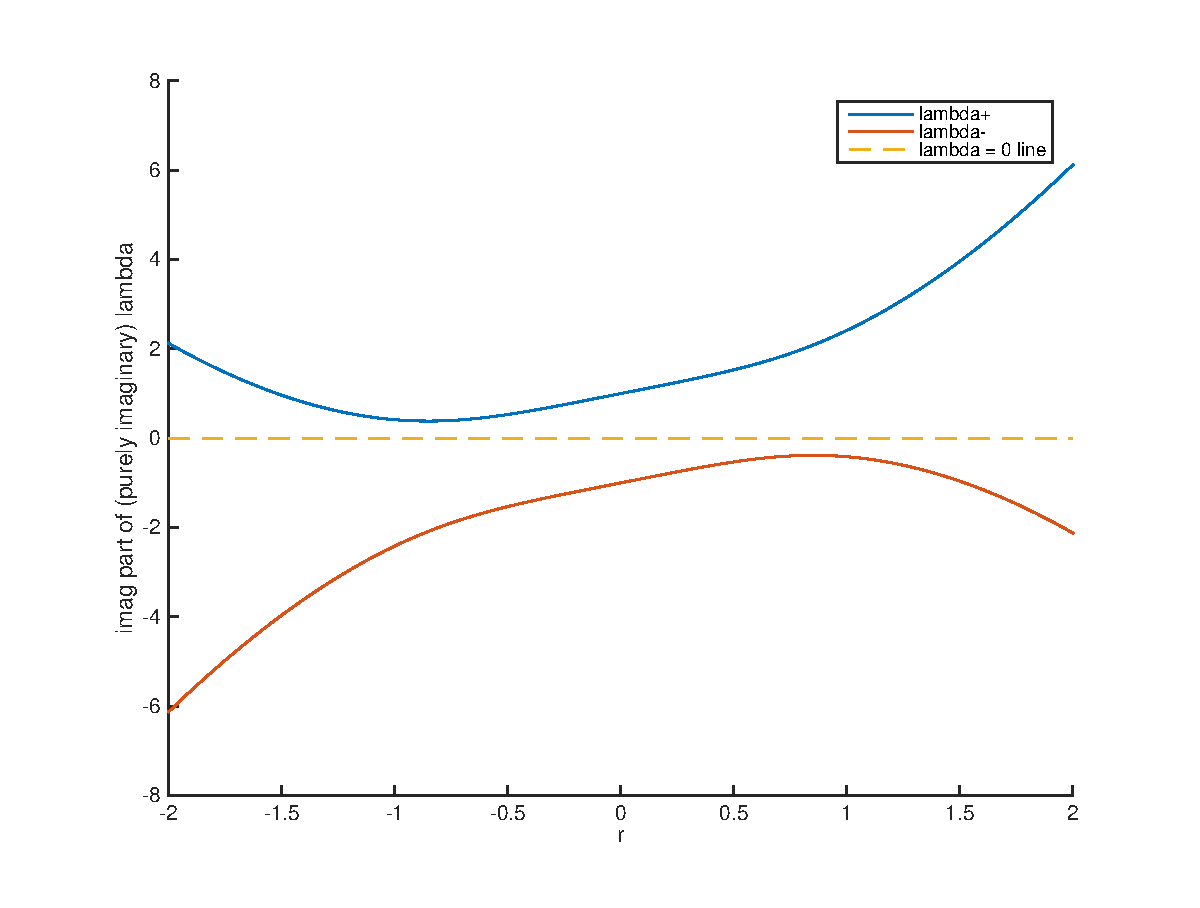
\includegraphics[width=10cm]{essspec1.eps}
\label{fig:essspec1}
\caption{Imaginary part of the purely imaginary essential spectrum for $c = 1$.}
\end{figure}

The equation for $\lambda(r)$ is of the form $\lambda_\pm(r) = k r \pm f(r^2)$. Since

\begin{align*}
\lambda_-(-r) = -kr - f((-r)^2) = -(kr + f(r^2)) = -\lambda_+(r)
\end{align*} 

and we take $r \in \R$, it suffices to look at $\lambda_+(r)$. Using Mathematica, we find

\begin{align*}
\lambda_+'(r) = c+\frac{2 r^3}{\sqrt{r^4+1}}
\end{align*}

Solving $\lambda_+'(r) = 0$ involves solving the 6th order polynomial

\[
4 r^6 - c^2 r^4 + c^2 = 0
\]

Mathematica will actually do it (!), but it is an epic mess. So we will look at it numerically using Matlab. The next plot shows the minimum value of $\lambda_+(r)$ as a function of $c$. Note that for $c = 0$ this minimum is clearly $0$, and for $c = \sqrt{2}$ it is not hard to show that this minimum is actually 0 (hence no essential spectrum gap). $c = \sqrt{2}$ is the bifurcation point mentioned above, so this is consistent.

\begin{figure}[H]
\centering
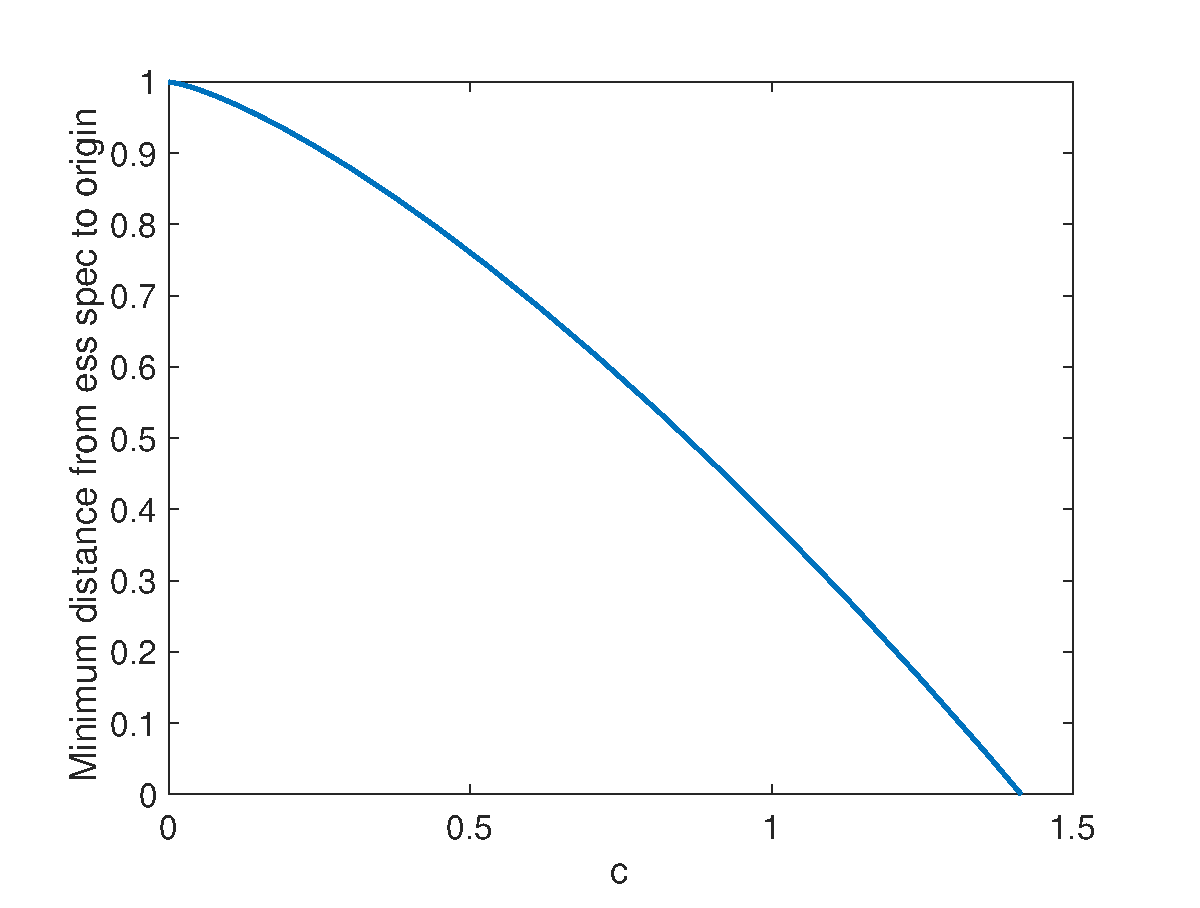
\includegraphics[width=10cm]{minlambdaplus.eps}
\label{fig:essspec2}
\caption{Minimum distance from essential spectrum to origin as a function of $c$.}
\end{figure}

Note that this minimum decreases strictly as $c$ increases, so the essential spectrum gap narrows (to 0) as $c$ increases from 0 to $\sqrt{2}$.\\

We could probably do better, i.e. approximate or get an exact formula (likely a nasty one) for this curve, but this is good enough for now.

\subsubsection{Point Spectrum}

Now that have looked at the essential spectrum, we can move on the point spectrum. At this point, there are only a few things we can say.\\

If $\lambda = 0$, the eigenvalue problem \eqref{quadeig} reduces to

\begin{equation*}
A_0(u_*) v = (\partial_x^4 + c^2 \partial_x^2 + e^{u_*})v = 0
\end{equation*}

Thus we are are interested in the kernel of $A_0$. If we take $v = \partial_x u_*$, then

\begin{align*}
A_0(u_*) \partial_x u_* &= 
(\partial_x^4 + c^2 \partial_x^2 + e^{u_*})\partial_x u_* \\
&= \partial_x[(u_*)_{xxxx} + c^2 (u_*)_{xx} + e^{u_*}] \\
&= \partial_x(1) \\
&= 0
\end{align*}

where we use the fact that $u_*$ is an equilibrium solution, thus must satisfy \eqref{eqODE}. Thus 0 is an eigenvalue of \eqref{evp} with corresponding eigenfunction $\partial_x u_*$.\\

Since the operator $A_0(u_*)$ is self-adjoint, by the Fredholm alternative we cannot have a function $v$ such that $A_0(u_*) v = \partial_x u_*$. (Otherwise $\partial_x u_*$ would be perpendicular to the kernel of $A_0(u_*)^* = A_0(u_*)$, which is impossible.) In other words, we cannot have a Jordan chain ending in $\partial_x u^*$.\\

Thus it makes sense to take the following hypothesis, which states that there is nothing else in the kernel of $A_0(u_*)$.

\begin{hypothesis}\label{kerA0hyp}
The kernel of $A_0(u_*)$ is given by
\begin{equation}\label{kerA0}
\ker A_0(u_*) = \spn\{ \partial_x u_*\}
\end{equation}
\end{hypothesis}

Finally, we look at the derivative with respect to the speed $c$, since it will be important in what is to follow. Taking the derivative of \eqref{eqODE} with respect to $c$, we get

\begin{align*}
0 &= u_{xxxxc} + 2 c u_{xx} + c^2 u_{xxc} + e^{u} u_c \\
&= 2 c u_{xx} + (\partial_x^4 + c^2 \partial_x^2 + e^{u})u_c
\end{align*}

At an equilibrium solution $u_*$, we rearrange this to get

\begin{align*}
(\partial_x^4 + c^2 \partial_x^2 + e^{u^*})u^*_c &= -2 c u^*_{xx}
\end{align*}

This simplifies to 

\begin{equation}\label{uc}
A_0(u_*) \partial_c u^* = -2 c u^*_{xx}
\end{equation}

For $\lambda \neq 0$, there is nothing else we can say now regarding the point spectrum. To locate the rest of the eigenvalues, we will have to use another technique, such as the Krein matrix or Lin's method.

\subsubsection{Numerics}

In this section, we compute the spectrum numerically with Matlab and the \texttt{quadeig} package. (Although Matlab has a built-in polynomial eigenvalue solver, \texttt{polyeig}, I decided to use the quadratic eigenvalue solver \texttt{quadeig} by Chris Munro, Sven Hammarling and Francoise Tisseu (2013) because they say it's better; it probably makes very little difference). For $c = 1.2$, here are plots of the spectrum of the linearization of \eqref{evp} about the single pulse solution $q(x; c)$. Matlab shows an essential spectrum gap, as discussed above, and predicts that this gap is $[-0.2061, 0.2061]$. The eigenvalue at 0 is from translation invariance, as discussed above.

\begin{figure}[H]
\centering
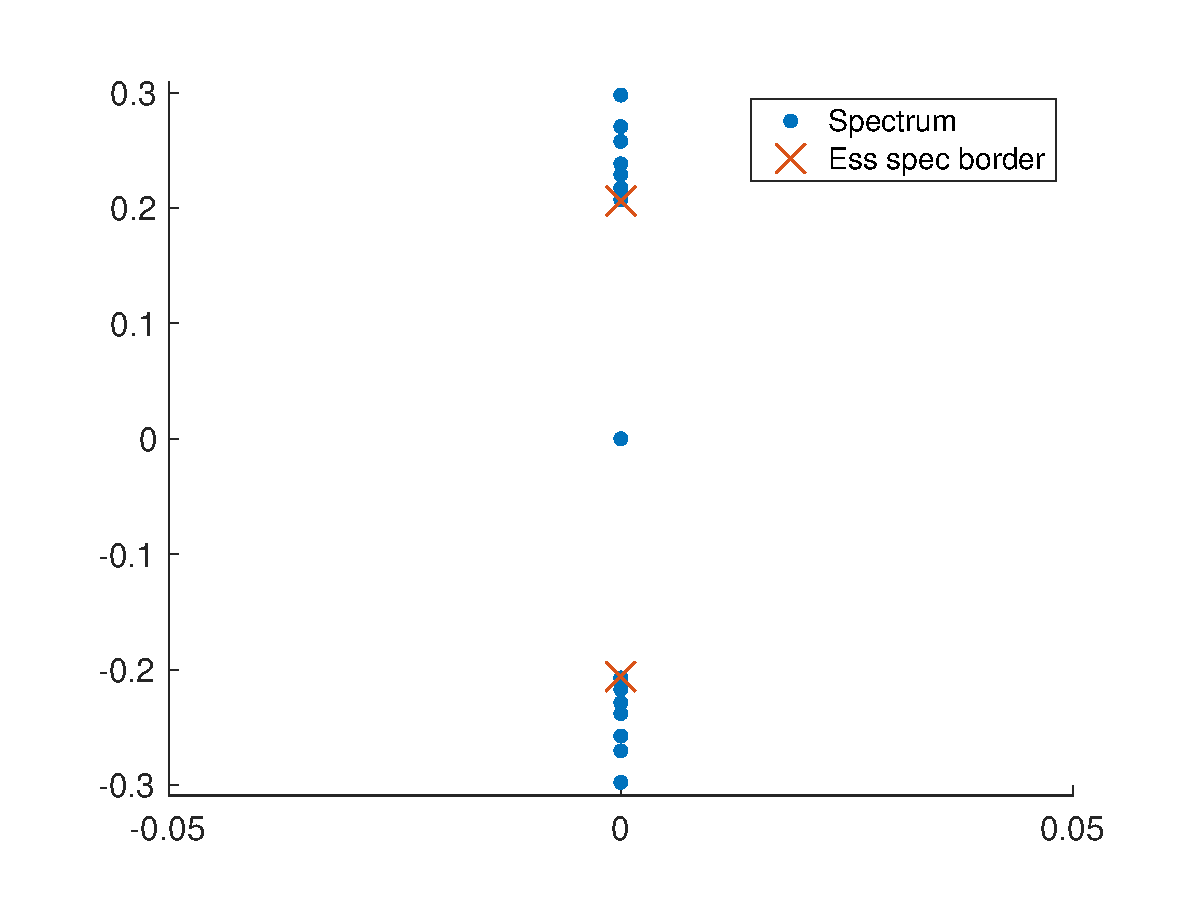
\includegraphics[width=8cm]{essspecboundsF256.eps}
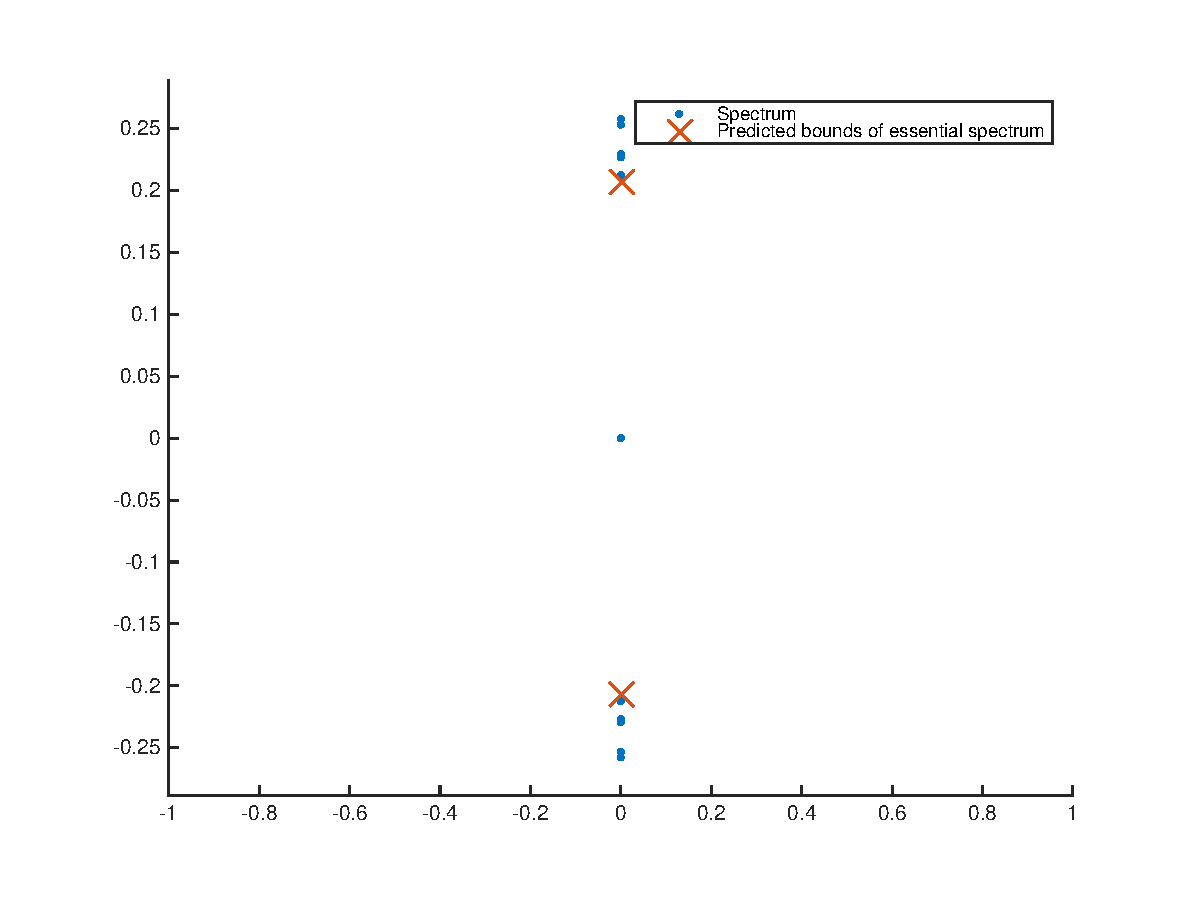
\includegraphics[width=8cm]{essspecboundsFD256.eps}
\caption{Essential spectrum gap for $c = 1.2$. Fourier spectral methods, $N = 256$ (left), finite difference methods, $N = 256$ (right)}
\end{figure}

\subsubsection{\texorpdfstring{Spectrum of $A_0(u_*)$}{}}

Next, we will look at the spectrum of the operator $A_0(u_*)$. Since $A_0(u_*)$ is self-adjoint, its spectrum will be real. First, we look at the essential spectrum. Writing the eigenvalue problem as a first order system, the operator $A_0(u_*)$ is given by

\begin{equation}\label{A0system}
\tilde{A}(\lambda; u_*) = \begin{pmatrix}
0 & 1 & 0 & 0 \\
0 & 0 & 1 & 0 \\
0 & 0 & 0 & 1 \\
\lambda - e^{u_*} & 0 & -c^2 & 0 
\end{pmatrix}
\end{equation}

Suppose $u^*$ is an equilibrium solution which is exponentially localized (as will be the case with all equilibrium solutions we will consider). By the Weyl Essential Spectrum Theorem, the essential spectrum only depends on the asymptotic matrix $\tilde{A}_\infty = \tilde{A}(\lambda; 0)$.

\begin{equation}
\tilde{A}_\infty = \begin{pmatrix}
0 & 1 & 0 & 0 \\
0 & 0 & 1 & 0 \\
0 & 0 & 0 & 1 \\
\lambda - 1 & 0 & -c^2 & 0 
\end{pmatrix}
\end{equation}

The characteristic polynomial of the asymptotic matrix $\tilde{A}_\infty$ is 

\[
p(\nu) = \nu^4 + c^2 \nu^2 - \lambda + 1
\]

For the essential spectrum, we take $\nu = i r$, where $r \in \R$. This becomes

\[
p(i r) = r^4 - c^2 r^2 - \lambda + 1 = 0
\]

Solving for $\lambda$ gives us

\[
\lambda(r) = r^4 - c^2 r^2 + 1 = r^2(r^2 - c^2) + 1
\]

This is a fourth-order polynomial with limits of $\infty$ at both ends, so all we need to do is find its minimum. Since $\lambda'(r) = 4 r^3 - 2 c^2 r = 2 r(2 r^2 - c^2)$, there will be a minimum when $r = c/\sqrt{2}$. At this minimum, $\lambda = 1 - c^4/4$. Thus, the essential spectrum of $A_0(u^*)$ is given by

\begin{equation}\label{A0ess}
\sigma_{\text{ess}}(A_0(u_*)) = [1 - c^4/4, \infty)
\end{equation}

For $c \in (0, \sqrt{2})$, which are the values of $c$ under consideration, the essential spectrum of $A_0(u_*)$ is positive and bounded away from the origin.\\

We discussed the kernel of $A_0(u_*)$ above. By Hypothesis \ref{kerA0hyp}, the kernel of $A_0(u_*)$ is one-dimensional and is spanned by $\partial_x u_*$. Thus we have a single eigenvalue of $A_0(u_*)$ at 0. \\

Any remaining eigenvalues will depend on the solution we are linearizing about. In what follows, will consider the linearization about a single-pulse homoclinic orbit $q(x; c)$. First, we compute the spectrum of $A_0(q)$ numerically.

\begin{figure}[H]
\centering
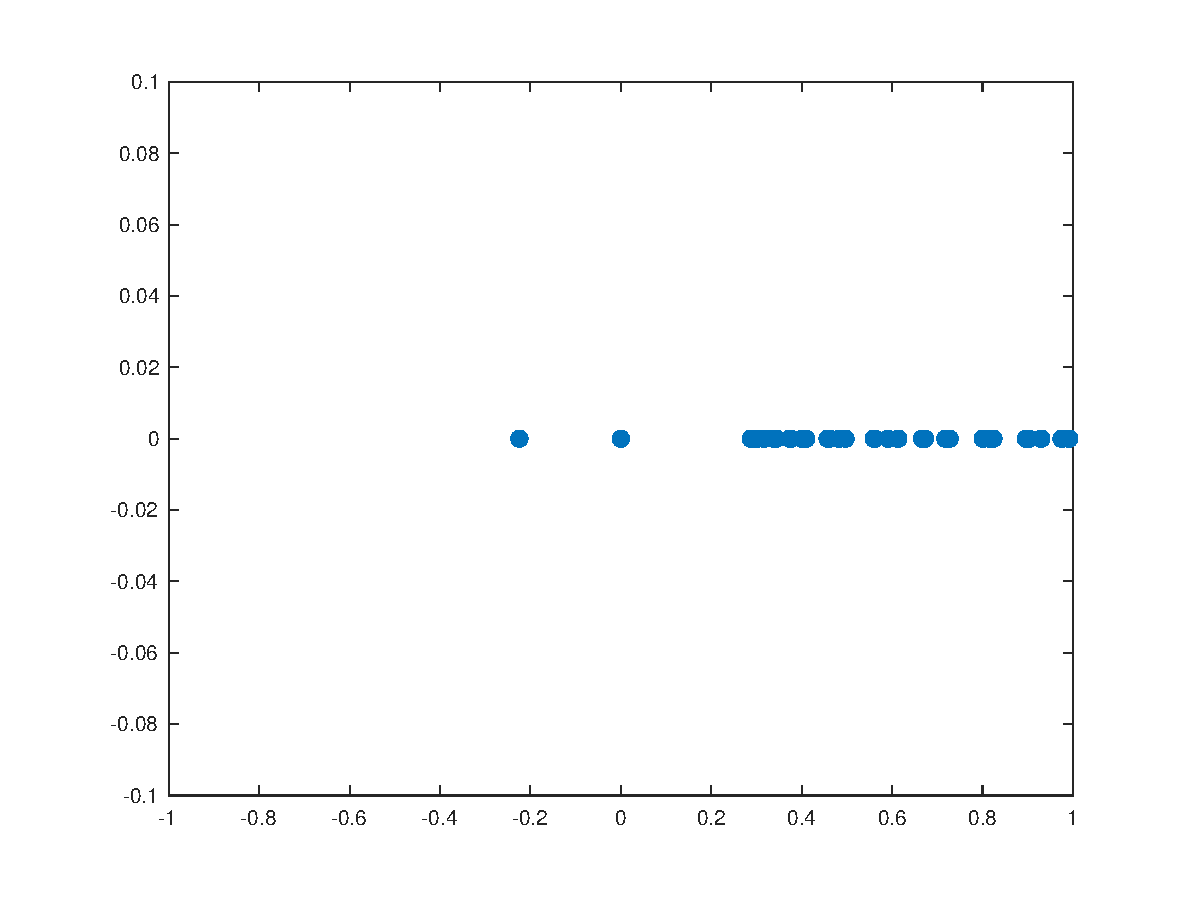
\includegraphics[width=8cm]{specA0.eps}
\caption{Spectrum of $A_0(q)$, the linearization about a single pulse $q$. $c = 1.3$. Finite difference methods, $N = 513$.}
\end{figure}

We see that there is a single eigenvalue at 0. We also see that the essential spectrum is positive, bounded away from 0, and is (approximately) given by \eqref{A0ess}. We also note the presence of a single negative eigenvalue.\\

In this case (as opposed to \cite{Sandstede1997}), it will be difficult (if not impossible) to prove the existence of a unique negative eigenvalue. The plot above suggests this is the case. In addition, we can compute numerically that $\langle A_0(q) q, q \rangle < 0$, so $A_0(q)$ is not positive definite. Thus we make the following hypothesis.

\begin{hypothesis}\label{A0neg}
For $c \in (0, \sqrt{2})$ and corresponding primary pulse $q(x; c)$, the operator $A_0(q)$ has exactly one negative eigenvalue $\lambda_- < 0$ with corresponding eigenfunction $v_-(x)$.
\end{hypothesis}

\subsection{Stability of Primary Pulse}

Choose a speed $c$ with $c^2 \in [0.5, 1.9]$, so that we can apply the results of \cite{Berg2018} and conclude that a symmetric homoclinic orbit $q(x; c)$ exists. To assess stability of this primary pulse, we follow \cite{Grillakis1987}.\\

Letting $v = u_t$, we can write \eqref{susp3} in the form 

\begin{equation}\label{2dsystem}
\frac{d \textbf{u} }{dt} = J E'(\textbf{u})
\end{equation}

where $\textbf{u} = \begin{pmatrix}u&v\end{pmatrix}^T$, $J$ is the standard symplectic matrix

\begin{equation*}
J = \begin{pmatrix}0 & 1 \\ -1 & 0 \end{pmatrix}
\end{equation*}

and $E(\textbf{u})$ is the energy

\begin{equation}\label{energy}
E(\textbf{u}) = \int_{-\infty}^\infty \left(\frac{1}{2} v^2 + \frac{1}{2}u_{xx}^2 + e^{u} - u \right)dx
\end{equation}

The energy $E$ is conserved (in $t$), since

\begin{align*}
\frac{d}{dt} E(\textbf{u}) &= \langle E'(\textbf{u}), \textbf{u}_t \rangle \\
&= \langle E'(\textbf{u}), J E'(\textbf{u}) \rangle \\
&= 0
\end{align*}

where the last equality holds because $J$ is skew-symmetric.\\

The equation \eqref{2dsystem} is invariant under the unitary translation group $T(s)$, defined by $T(s)\phi(\cdot) = \phi(\cdot - s)$. It is easy to see that $T^*(s) = [T(s)]^{-1} = T(-s)$. The infinitesimal generator of $T(s)$ is

\begin{equation}
T'(0) = \begin{pmatrix}\partial_x & 0 \\ 0 & \partial_x \end{pmatrix}
\end{equation}

The energy $E(\textbf{u})$ is also invariant under $T(s)$, i.e. $E(T(s) \textbf{u}) = E(\textbf{u})$ for all $s \in \R$. This is clear since \eqref{energy} does not involve $x$ directly, and we are integrating over $\R$. If we differentiate $E(T(s) \textbf{u}) = E(\textbf{u})$ with respect to $s$ at $s = 0$, we obtain the relation

\begin{equation}\label{IP1}
\langle E'(\textbf{u}), T'(0) \textbf{u} \rangle = 0
\end{equation}

As in \cite{Grillakis1987}, we define 

\begin{equation}\label{defB}
B = J^{-1} T'(0) = \begin{pmatrix}0 & -\partial_x \\ \partial_x & 0\end{pmatrix}
\end{equation}

Since $B$ is the product of two skew-symmetric operators, $B$ is self-adjoint. Using this, we define the momentum as

\begin{equation}\label{defQ}
Q(\textbf{u}) = \frac{1}{2}\langle B \textbf{u}, \textbf{u} \rangle
\end{equation}

It is not hard to show that $Q'(\textbf{u}) = B \textbf{u}$. Expanding \eqref{defQ} and integrating by parts, we get

\begin{align*}
Q(\textbf{u}) &= \frac{1}{2}\langle (-v_x, u_x), (u, v) \rangle \\
&= \frac{1}{2} \left( -\int_{-\infty}^\infty v_x u dx + \int_{-\infty}^\infty u_x v dx \right) \\
&= \int_{-\infty}^\infty u_x v dx
\end{align*}

The momentum $Q(\textbf{u})$ is also conserved in $t$, since

\begin{align*}
\frac{d}{dt} E(\textbf{u}) &= \langle Q'(\textbf{u}), \textbf{u}_t \rangle \\ 
&= \langle B \textbf{u}, J E'(\textbf{u}) \rangle \\
&= -\langle J B \textbf{u}, E'(\textbf{u}) \rangle \\
&= -\langle T'(0) \textbf{u}, E'(\textbf{u}) \rangle \\
&= 0
\end{align*}

where we used \eqref{defB} and \eqref{IP1}.\\

To show that the primary pulse $q(x; c)$ is stable, we will use Theorem 3 in \cite{Grillakis1987}. To do this, we need to verify the assumptions of the theorem. Assumption 1 concerns existence of solutions to \eqref{2dsystem}. We will take this as a hypothesis (unless we can find a reference to this somewhere. Chen and McKenna do not look at this).

\begin{hypothesis}
For every initial condition $\textbf{u}_0$ there exists a solution $\textbf{u}(t)$ to \eqref{2dsystem} on the interval $I = [0, T]$, where $T$ only depends on $||\textbf{u}_0||$, such that $\textbf{u}(0) = \textbf{u}(0)$. 
\end{hypothesis}

Assumption 2 in \cite{Grillakis1987} involves bound states, which are special solutions of the form

\begin{equation}\label{boundstate}
\textbf{u}(x, t) = T(ct)\boldsymbol\phi(x) = \boldsymbol\phi(x - ct)
\end{equation}

(We use the variable $c$ to represent speed instead of $\omega$). By p. 166 of \cite{Grillakis1987}, if $\boldsymbol\phi(x) $ satisfies the stationary equation

\begin{equation}\label{boundstateeq}
E'(\boldsymbol\phi) - c Q'(\boldsymbol\phi) = 0
\end{equation}

then $T(ct)\boldsymbol\phi$ is a bound state. Writing $\boldsymbol\phi = \begin{pmatrix}\phi&\psi\end{pmatrix}^T$, in our case this becomes the pair of equations

\begin{align*}
\phi_{xxxx} + c \psi_x + e^{\phi} - 1 &= 0 \\
\psi - c \phi_x &= 0
\end{align*} 

Substituting the second equation into the first gives us

\begin{equation}
\phi_{xxxx} + c^2 \psi_{xx} + e^{\phi} - 1 = 0
\end{equation}

Since this is the same as \eqref{eqODE}, $\phi = q(x; c)$ is a bound state solution to \eqref{boundstateeq}. Let $\textbf{q}(x; c) =\begin{pmatrix}q(x; c) &c q_x(x; c) \end{pmatrix}$. By smooth dependence on parameters, since \eqref{eqODE} is smooth in $c$, the map $c \mapsto \textbf{q}(x; c)$ is smooth in $c$. Since the solution $\textbf{q}(x; c)$ is smooth, part (c) in Assumption 2 of \cite{Grillakis1987} is satisfied, i.e. $\textbf{q}(x; c) \in D(T'(0)^3) \cap D(J I T'(0)^2)$. Finally, since none of the derivatives in $x$ of $\textbf{q}(x; c)$ are 0, $T'(0)q(x; c) \neq 0$. Thus Assumption 2 in \cite{Grillakis1987} is satisfied.\\

Finally, as in \cite{Grillakis1987}, we define the scalar

\begin{equation}\label{defd}
d(c) = E(\textbf{q}(x; c)) - c Q(\textbf{q}(x; c))
\end{equation}

and the operator 

\begin{equation}\label{defHc}
H_c = E''(\textbf{q}(x; c)) - c Q''(\textbf{q}(x; c))
\end{equation}

For this particular problem, we have

\begin{equation}
H_c = \begin{pmatrix}
\partial_x^4 + e^q & c \partial_x \\
-c \partial_x & 1
\end{pmatrix}
\end{equation}

We will verify Assumption 3B instead of Assumption 3. (This is suggested in the errata at the end of \cite{Grillakis1990}). For $\textbf{u} = \begin{pmatrix}u & v\end{pmatrix}^T$, 

\begin{align*}
\langle H_c \textbf{u}, \textbf{u} \rangle
&= \langle \begin{pmatrix} (\partial_x^4 + e^q)u + c \partial_x v \\ -c \partial_x u + v  \end{pmatrix},
\begin{pmatrix} u \\ v \end{pmatrix} \rangle \\ 
&= \langle (\partial_x^4 + e^q)u + c \partial_x v, u \rangle + \langle -c \partial_x u + v, v\rangle \\
&= \langle (\partial_x^4 + e^q)u, u \rangle + c \langle \partial_x v, u \rangle + c \langle -\partial_x u, v \rangle + \langle v, v \rangle \\
&= \langle (\partial_x^4 + e^q)u, u \rangle + c^2 \langle \partial_x^2 u, u \rangle - 2 c \langle \partial_x u, v \rangle + \langle v, v \rangle - c^2 \langle \partial_x^2 u, u \rangle\\
&= \langle A_0 u, u \rangle + \langle v, v \rangle - 2 c \langle v, \partial_x u \rangle + c^2 \langle \partial_x, \partial_x u \rangle\\
&= \langle A_0 u, u \rangle + || v - c \partial_x u||^2
\end{align*}

By Hypothesis \ref{A0neg}, $A_0$ has exactly one negative eigenvalue $\lambda_- < 0$ with corresponding eigenfunction $v_-(x)$. Let $\textbf{u} = \begin{pmatrix} v_-(x), c \partial_x v_-(x) \end{pmatrix}^T$. Substituting this in, we obtain

\begin{align*}
\langle H_c \textbf{u}, \textbf{u} \rangle &=
\langle A_0 v_-, v_- \rangle + || c \partial_x v_- - c \partial_x v_-||^2 \\
&= \lambda_- ||v_-||^2 < 0
\end{align*}

which verifies part (i) of Assumption 3B.\\

Next, we find kernel of $H_c$ by solving $H_c \textbf{u} = 0$. This is equivalent to solving the system of equations

\begin{align*}
u_{xxxx} + e^q u + c v_x &= 0 \\
-c u_x + v &= 0
\end{align*}

Multiplying the second equation by $c$, differentiating with respect to $x$, and substituting it into the first equation, we get

\begin{equation}
(\partial_x^4 + c^2 \partial_x^2 + e^q)u = 0
\end{equation}

which, in the notation of the previous section is

\begin{equation}
A_0(q) u = 0
\end{equation}

By Hypothesis \ref{kerA0hyp}, the kernel of $A_0(q)$ is spanned by $\partial_x q$, thus the kernel of $H_c$ is spanned by $\begin{pmatrix} \partial_x q, c \partial_x^2 q \end{pmatrix}$. Define the subspace $N$ by

\begin{equation}
N = \spn\{ \partial_x q, v_-\}
\end{equation}

i.e. $N$ is the span of all eigenfunction of $A_0$ which correspond to eigenvalues which are not positive. Then define the space

\begin{equation}
\tilde{N} = \left\{
\begin{pmatrix}u & v\end{pmatrix}^T : u \in S^\perp, v = 0
\right\}
\end{equation}

Then $\tilde{N}$ is a closed subspace. For any $\textbf{u} = \begin{pmatrix}u & 0\end{pmatrix}^T \in \tilde{N}$, since $A_0(q)$ is positive definite on $N^\perp$, there exists a constant $\delta > 0$ such that $\langle A_0 u, u \rangle \geq \delta ||u||^2$. Thus we have for $\textbf{u} \in \tilde{N}$,

\begin{align*}
\langle H_c \textbf{u}, \textbf{u} \rangle 
&= \langle A_0(q) u, u \rangle + || -c \partial_x u||^2 \\
&\geq \delta ||u||^2\\
&= \delta ||\textbf{u}||^2
\end{align*}

This verifies part (ii) of Assumption 3B. Part (iii) holds since $v_-$ and $q_x$ are linearly independent. Having verified Assumptions 1, 2, and 3B, we can invoke Theorem 3 of \cite{Grillakis1987} to conclude that $q(x)$ is stable if and only if $d''(c) > 0$. Differentiating \eqref{defd}, we have

\begin{align*}
d'(c) &= E'(\textbf{q})\partial_c \textbf{q} - Q(\textbf{q}) - c Q'(\textbf{q}) \partial_c \textbf{q} \\
&= [E'(\textbf{q}) - c Q'(\textbf{q})]\partial_c \textbf{q} - Q(\textbf{q}) \\
&= - Q(\textbf{q}) \\
&= -\int_{-\infty}^\infty q_x c q_x dx \\
&= -c ||q_x||^2
\end{align*}

since $E'(\textbf{q}) - c Q'(\textbf{q}) = 0$ by \eqref{boundstateeq}, since $\textbf{q}$ is a bound state. Differentiating once more, we have

\begin{align*}
d''(c) &= -\frac{\partial}{\partial c} \left( c ||q_x||^2 \right)
\end{align*}

Thus we can state the following proposition.

\begin{proposition}\label{stabcrit}
Let $c \in [\sqrt{0.5}, \sqrt{1.9}]$, and let $q(x; c)$ be the symmetric homoclinic orbit (single pulse) solution to \eqref{eqODE} associated with this speed $c$. Then $q(x)$ is stable if and only if $d''(c) > 0$, where

\begin{equation}\label{dcc}
d''(c) = -\frac{\partial}{\partial c} \left( c ||q_x||^2 \right)
\end{equation}
\end{proposition}

In our case, numerics suggest that $d''(c) > 0$, so $q(x; c)$ is stable. Thus we make the following hypothesis.

\begin{hypothesis}\label{hypdccpos}
$d''(c) > 0$ for $c \in [\sqrt{0.5}, \sqrt{1.9}]$.
\end{hypothesis}


\subsection{Multipulse Solutions}

\subsubsection{Existence}

Let $c \in [\sqrt{0.5}, \sqrt{1.9}]$ and let $q(x; c)$ be the symmetric homoclinic orbit solution to \eqref{eqODE}. We take the following hypothesis regarding the primary pulse.

\begin{hypothesis}\label{transverseq}
The primary pulse $q(x; c)$ is transversely constructed, i.e. 
\[
T_{q(0; c} W^s(0; c) \cap T_{q(0; c} W^u(0; c) = \R q'(0; c).
\]
\end{hypothesis}

Recall that 0 is a hyperbolic equilibrium for \eqref{eqODE} and that \eqref{eqODE} is a Hamiltonian system. Then, using Lin's method (San93, \cite{Sandstede1998}, \cite{Sandstede1997}), we can construct an $n-$pulse which resembles, to leading order, $n$ copies of the primary pulse $q$ joined together. The $n$ peaks of $q_n$ are separated by distances $2 X_1, \dots, 2 X_{n-1}$. We can write $q_n$ as 

\begin{align}\label{qn}
q_n = \sum_{i = 1}^{n} q^i + r
\end{align}

where each function $q^i$ is a translate of the primary pulse $q$ a signed distance $L_i$, i.e. 

\begin{equation}\label{qi}
q^i(\cdot) = q(\cdot - L_i)
\end{equation}

From Lin's method, the translates $q^i$ and all their derivatives are exponentially separated. We also get from Lin's method a uniform bound on the remainder term $r$.

\begin{equation}
||r|| \leq C e^{-\alpha X_m}
\end{equation}

where

\begin{equation}\label{defXm}
X_m = \min\{X_1, \dots, X_n \}
\end{equation}

This bound holds for all derivatives with respect to $x$ (see Theorem 1 in \cite{Sandstede1998}). Since everything is translation invariant, we do not need to define a ``center'' for the multipulse. For $i, j = 1, \dots, n$, let $\rho_{ji}$ be the signed distance between peak $i$ and peak $j$, i.e. 

\begin{equation}\label{rhoji}
\rho_{ji} = L_j - L_i
\end{equation}

Then for all $i, j$, $|\rho_{ji}| \geq 2 X_m$.\\

Using Lin's method again (following \cite{Sandstede1998}), we can show that $A_0(q_n)$ has $n$ distinct small eigenvalues near 0 (this includes one eigenvalue at 0 corresponding to the kernel eigenfunction $\partial_x q_n$). Let $\{\nu_1, \dots, \nu_n\}$ be these small eigenvalues, and let $\{s_1, \dots, s_n \}$ be the corresponding eigenfunctions. We number these so that $\nu_1 = 0$. Since $A_0$ is self-adjoint and the eigenvalues $\nu_i$ are distinct, the eigenfunctions $s_i$ are orthogonal. Since we can scale the eigenfunctions any way we like, we will take

\begin{equation}\label{orthonormaleigs}
\langle s_i, s_j \rangle = ||q_x(x; c)||^2 \delta_{ij}
\end{equation}

From Lin's method, these eigenvalues are small. In particular, we have for $i = 1, \dots, n$

\begin{equation}
|\nu_i| = \mathcal{O}(e^{-2 \alpha X_m})
\end{equation}

From Lin's method (\cite{Sandstede1998}), the eigenfunctions $s_i$ are, to leading order, linear combinations of translates of the derivative of the primary pulse. In other words, for $j = 1, \dots, n$

\begin{align}\label{sj}
s_j = \sum_{i = 1}^{n} d_{ji} q^i_x + w_j
\end{align}

for constants $d_{ji} \in \C$, where the $q^i$ are defined above. Let $D$ be the matrix defined by 

\begin{equation}\label{matrixD}
(D)_{ji} = d_{ji}
\end{equation}

(Note that this is not the same matrix $D$ as in \cite{Sandstede1998}). For the remainder terms, we have from Lin's method the uniform bound

\begin{equation}\label{sjwbound}
||w_j|| \leq C e^{-2 \alpha X_m}
\end{equation}

which also holds for derivatives with respect to $x$.

\subsubsection{Numerics}

In this section, we numerically construct multipulse solutions to \eqref{eqODE}. We start by constructing the primary pulse. Unlike systems such as KdV5, we do not have an exact solution to \eqref{eqODE} for any value of $c$, thus we cannot do parameter continuation. Nevertheless, using a variant of the mountain pass and string methods which combines \cite{Chen1997} and \cite{Chamard2011}, we can construct a primary pulse as follows.

\begin{enumerate}
	\item The energy functional $I \in C^1(H^2, \R)$ is given by
	\begin{equation}
	I(z) = \frac{1}{2} \int_\R (|z''|^2 - c^2 |z'|^2)dx 
	+ \int_\R (e^z - z - 1) dx
	\end{equation}
	where $z$ is a function of $x$. For the numerical method, we truncate the domain to $[-L, L]$ for $L$ large.
	\item To do the mountain pass method, we need to find
	\begin{enumerate}
		\item A function $e_1 \in H^2$ which is a local minimum of $I$. From Lemma 2.4 in \cite{Chen1997}, $e_1 = 0$ satisfies this.
		\item A function $e_2 \in H^2$ for which $I(e_2) < I(e^1) = I(0) = 0$. We can use Lemma 2.5 in \cite{Chen1997} to find such an $e_2$. 
	\end{enumerate} 
	The solution we want, by the Mountain Pass Lemma, is the infimum of the maxima of $I$ along all paths joining $e_1$ and $e_2$.
	\item Choose a discretization scheme. Following \cite{Chen1997}, we use the finite difference method.
	\item We then use the String Method from \cite{Chamard2011}.
	\begin{enumerate}
		\item Join $e_1$ and $e_2$ by a piecewise linear path $U(t) = t e_1 + (1-t) e_2 = (1-t)e_2$. Choose a discrete set of values for $t$ which are evenly spaced, i.e. the $N+1$ values $t = [0, 1/N, 2/N, ..., 1]$ for some reasonably sized $N$. We ended up using $N = 10$, which worked fine.
		\item Reparameterize the path to get points more-or-less equidistantly distributed in the $H^1$ norm.
		\item Evaluate the steepest decent direction $v(t_i)$ for all points $U(t_i)$ along the path. The steepest descent direction is computed as in section 3 of \cite{Chen1997}.
		\item For constrained maximal step size $h_M$, perform gradient descent on all points on the path $U(t_i)$ in the direction of $v(t_i)$.
		\item Go back to the reparameterization step, and repeat all this a bunch of times. Theoretically there is a termination condition, but we don't actually need to worry about that since we will be using Matlab's \texttt{fsolve}.
	\end{enumerate}
	\item After doing this a bunch of times, take the element of the path for which $I(U(t_i))$ is maximum. Or take one close to the maximum. Use this as an initial guess for Matlab's \texttt{fsolve}. This should converge to the solution we are looking for.
\end{enumerate}

Here are plots of the primary pulse $q(x; c)$ found using this method for $c = 1.354$ and $c = 1.40$. Compare these to figure 3 on p. 347 of \cite{Chen1997}. Note that by the substitution we performed, the baseline in our plots is at 0 as opposed to 1 in \cite{Chen1997}.

\begin{figure}[H]
\centering
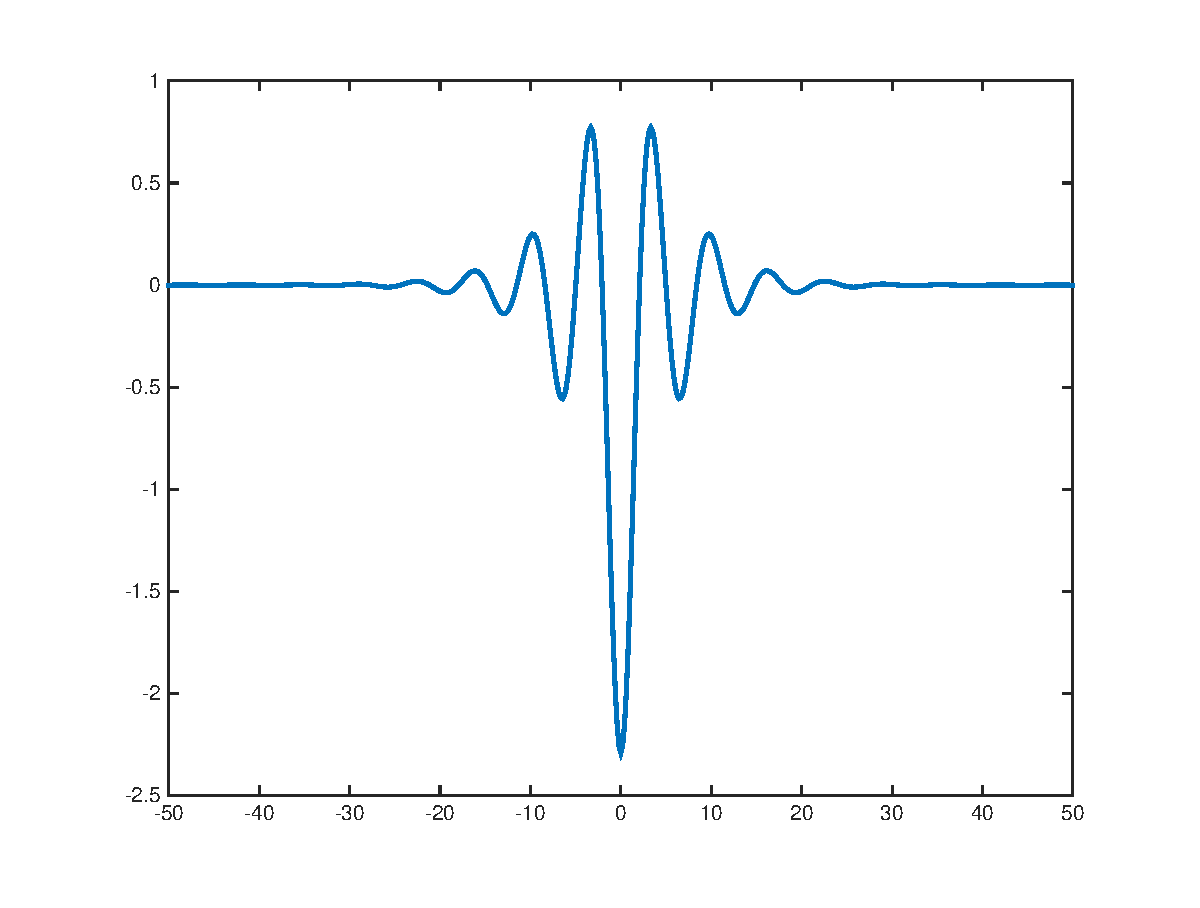
\includegraphics[width=8cm]{single1354.eps}
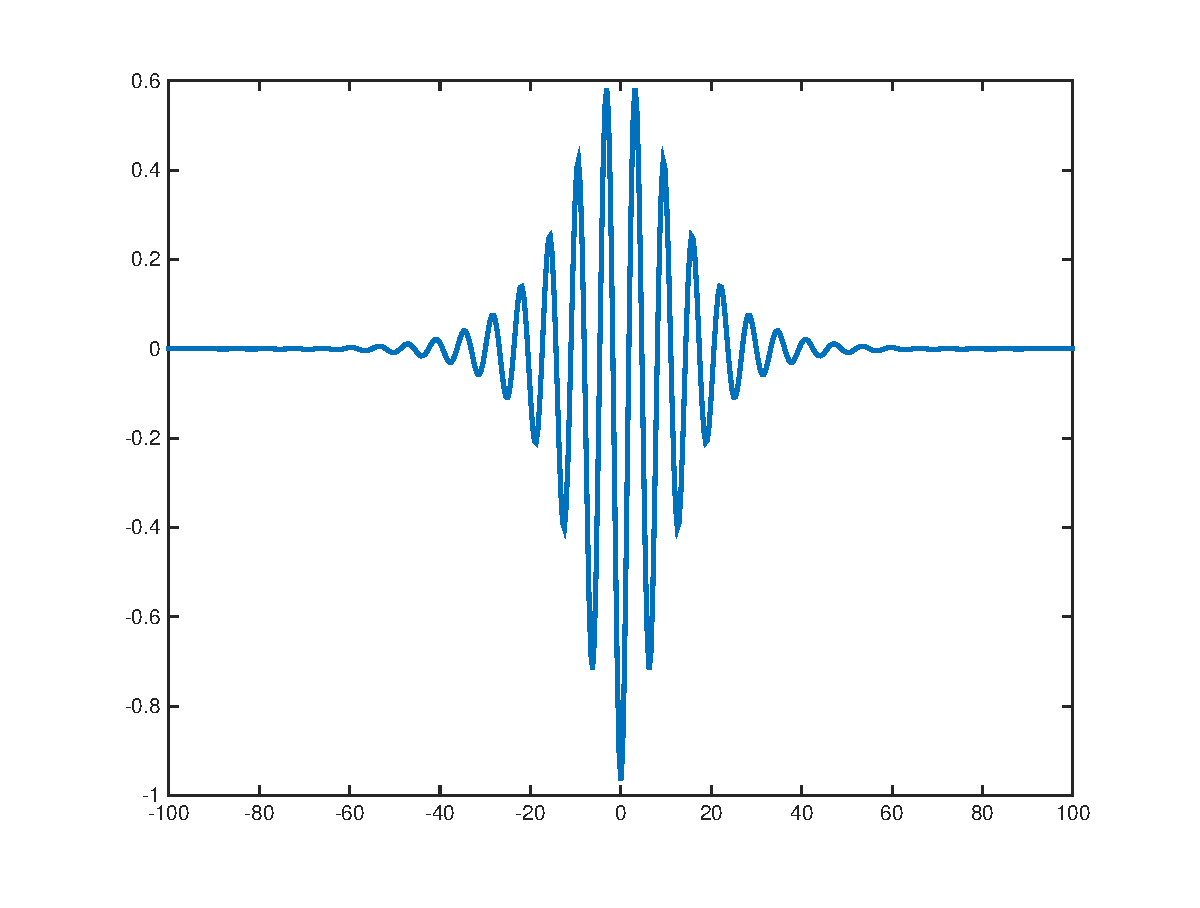
\includegraphics[width=8cm]{single14.eps}
\label{fig:single1}
\caption{Primary pulse solutions $q(x;c)$ to \eqref{eqODE}. $c = 1.354$ (left) and $c = 1.40$ (right).}
\end{figure}

We also compute solutions for other values of $c$.

\begin{figure}[H]
\centering
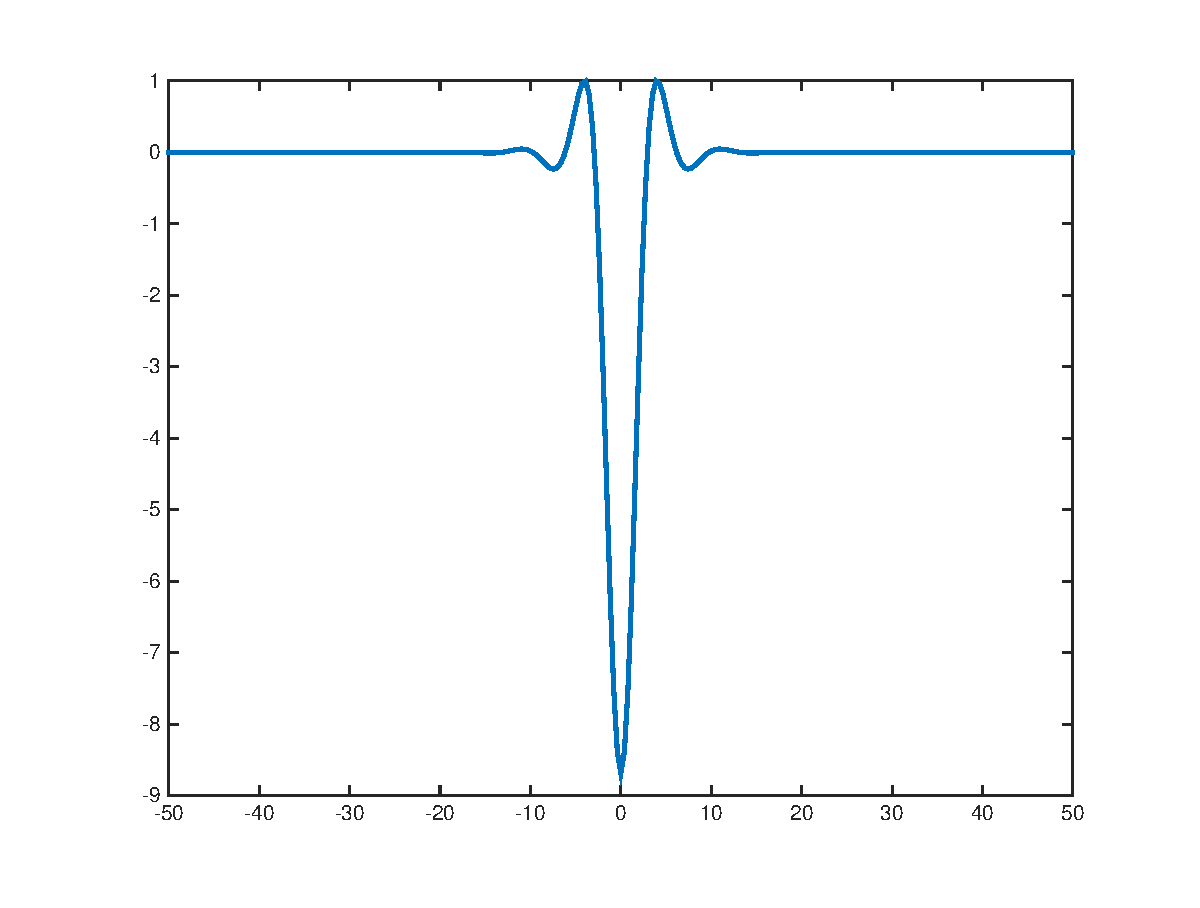
\includegraphics[width=8cm]{single11.eps}
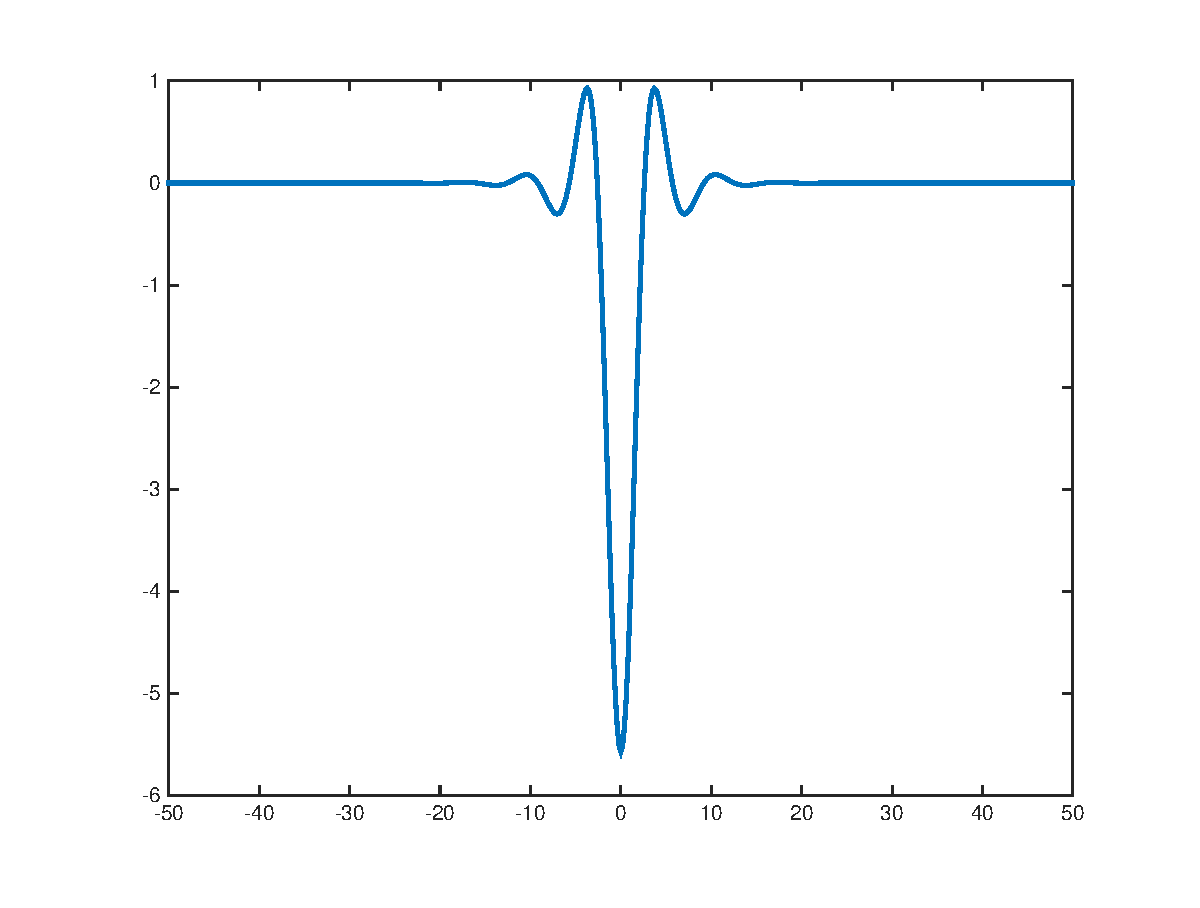
\includegraphics[width=8cm]{single12.eps}
\label{fig:single2}
\caption{Primary pulse solutions $q(x;c)$ to \eqref{eqODE}. $c = 1.1$ (left) and $c = 1.2$ (right).}
\end{figure}

Let $\nu = \pm \alpha \pm i \beta$ be the eigenvalues of the linearization about the zero solution. Then we can show numerically that the tail decays exponentially with rate (approximately) $\alpha$, and the period of the tail oscillations is (approximately) $2 \pi / \beta$. This is what we expect. \\

Now that we have constructed the primary pulse, we can join the tails to form double pulses. This join can only be performed every quarter period, i.e. every $\pi / 2 \beta$, so this produces a countable family of double pulses. After gluing two primary pulses together at the approprate interval and using Matlab's \texttt{fsolve} function, here are the first four double pulses for $c = 1.2$.

\begin{figure}[H]
\centering
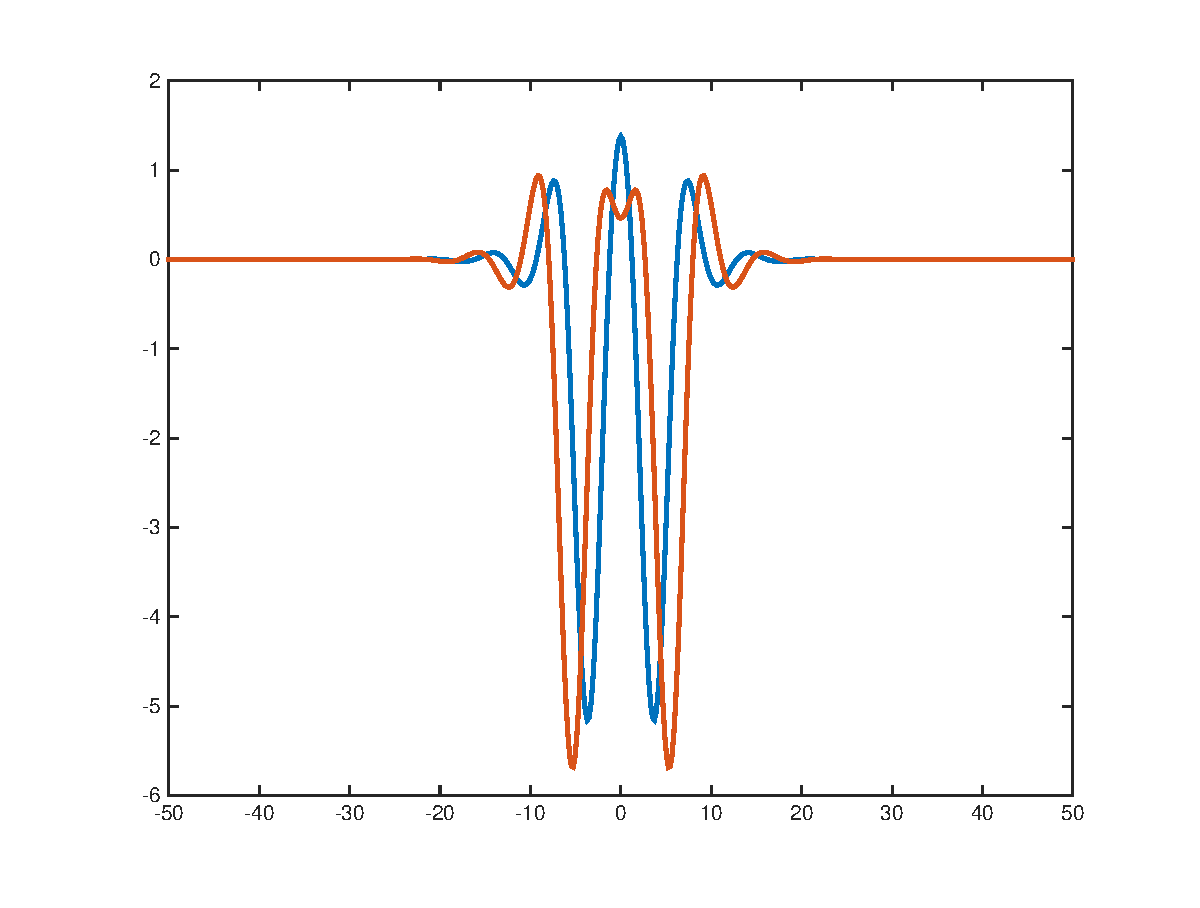
\includegraphics[width=8cm]{double12_12.eps}
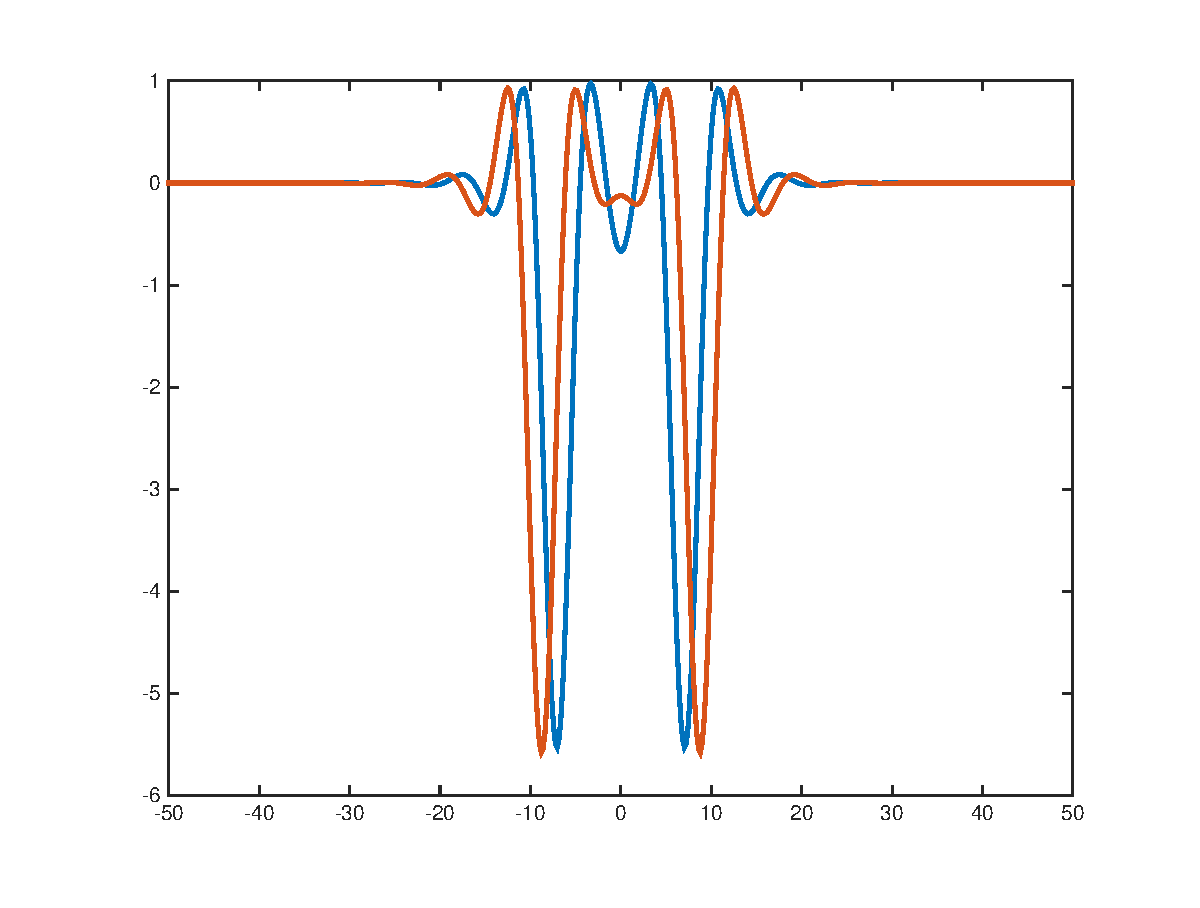
\includegraphics[width=8cm]{double12_34.eps}
\caption{Double pulse traveling wave solutions to \eqref{eqODE} for $c = 1.2$. Double pulses 1 and 2 (left). Double pulses 3 and 4 (right).}
\end{figure}

We can similarly numerically construct $n-$pulses for any $n$. Note that these multipulses do not have to be symmetric. We can also obtain periodic versions of these by interpolating the finite difference solutions onto the appropriate periodic grid, writing the operators using Fourier spectral matrices, and using \texttt{fsolve}. This is not shown.\\

\subsection{Eigenvalue Computation, Numerics}

In this section, we compute the eigenvalues numerically for the linearization about the multipulse solutions which we just constructed. First, we look at the eigenvalues of $A_0(q_2)$ for the first two double pulses.

\begin{figure}[H]
\centering
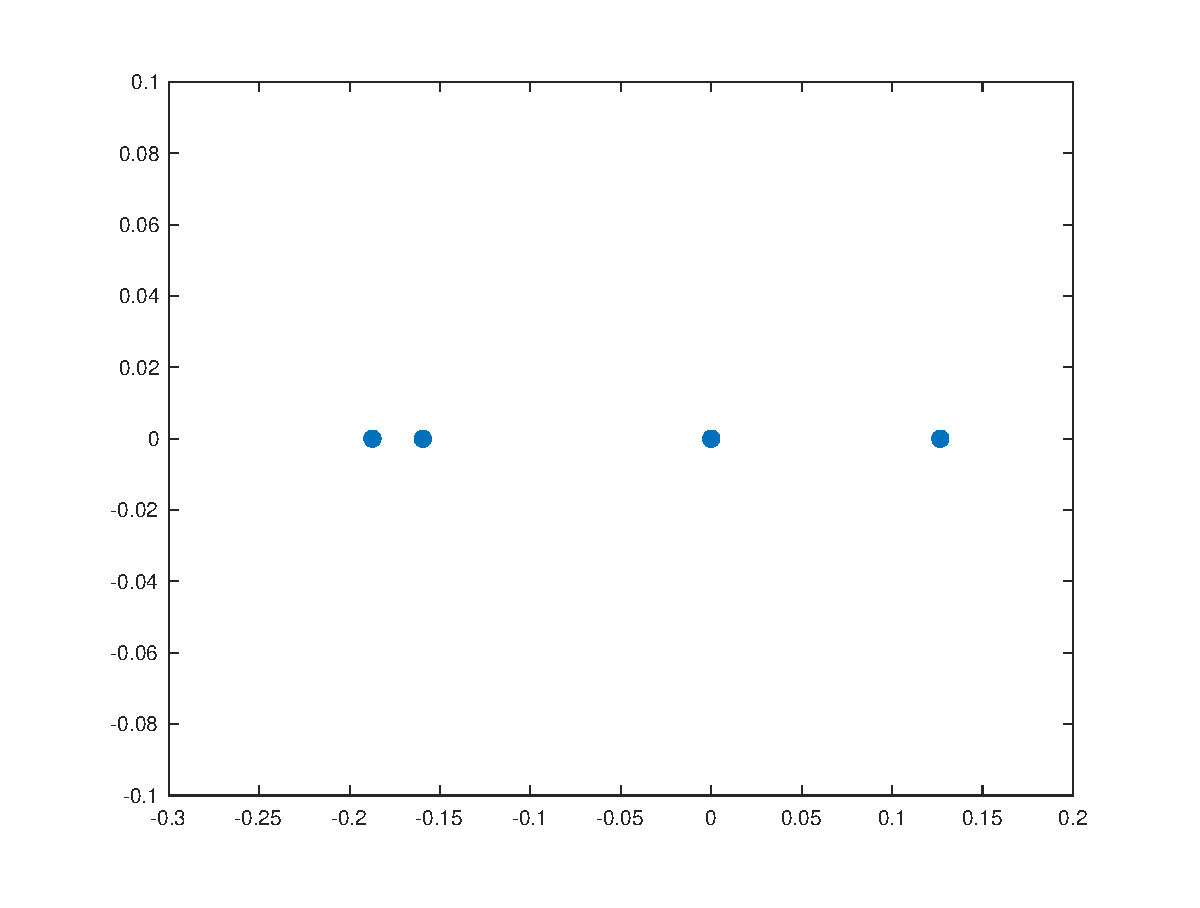
\includegraphics[width=8cm]{specA0d1}
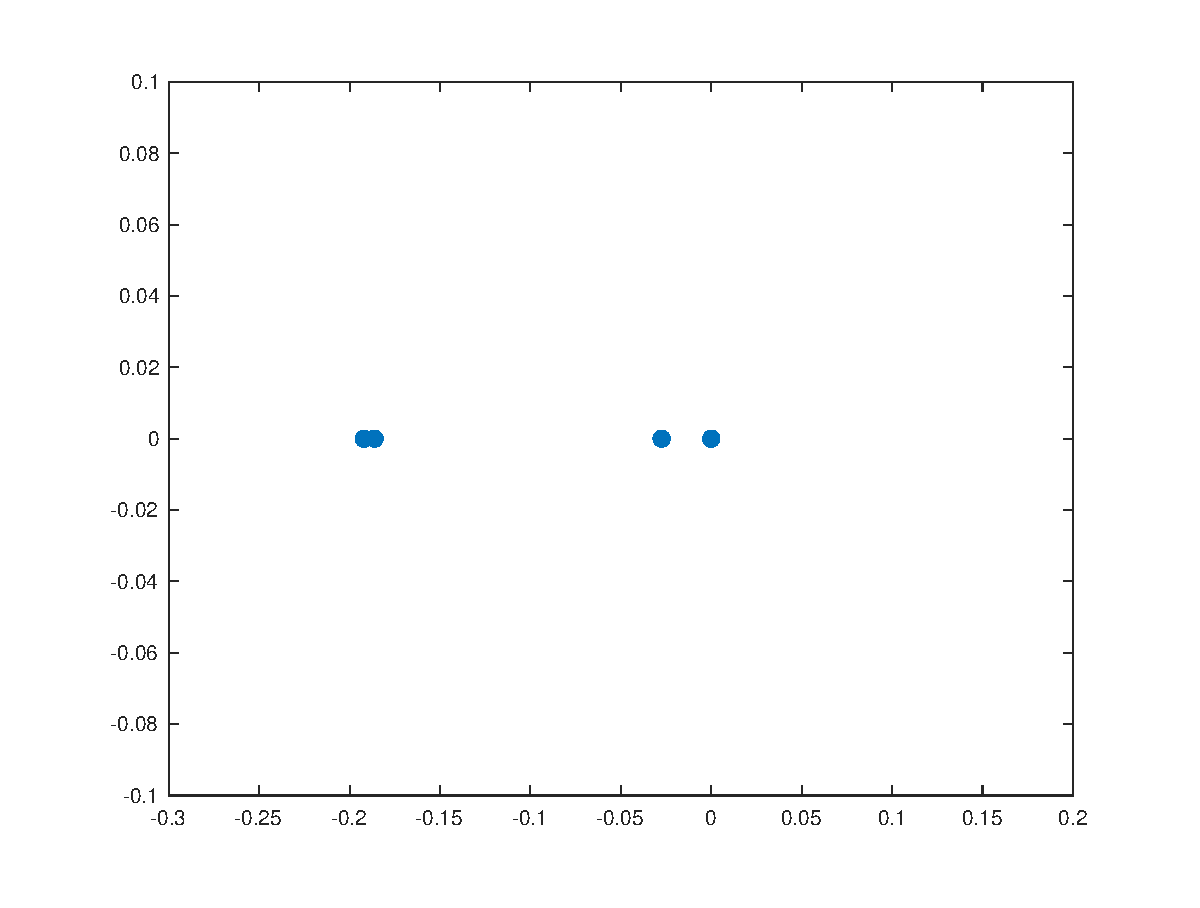
\includegraphics[width=8cm]{specA0d2}
\caption{Eigenvalues of $A_0(q_2)$ for $c = 1.2$. Double pulses 1 (left) and double pulses 2 (right).}
\end{figure}

Note that there are two small eigenvalues near 0 and a clump of two negative eigenvalues. In essence, the eigenvalues for $A(q)$ have each split into a pair. Note that for double pulse 1, the small eigenvalue near 0 is positive, whereas for double pulse 2, this eigenvalue is negative. This pattern of alternating positive and negative eigenvalues continues as we go to higher double pulses.\\

Next, we look at the eigenvalues of the quadratic eigenvalue problem \eqref{quadeig}. For double pulse 1, here is the spectrum (zoomed near the origin) and a plot of the eigenfunctions corresponding to the small interaction eigenvalues. Note there is a pair of real interaction eigenvalues.

\begin{figure}[H]
\centering
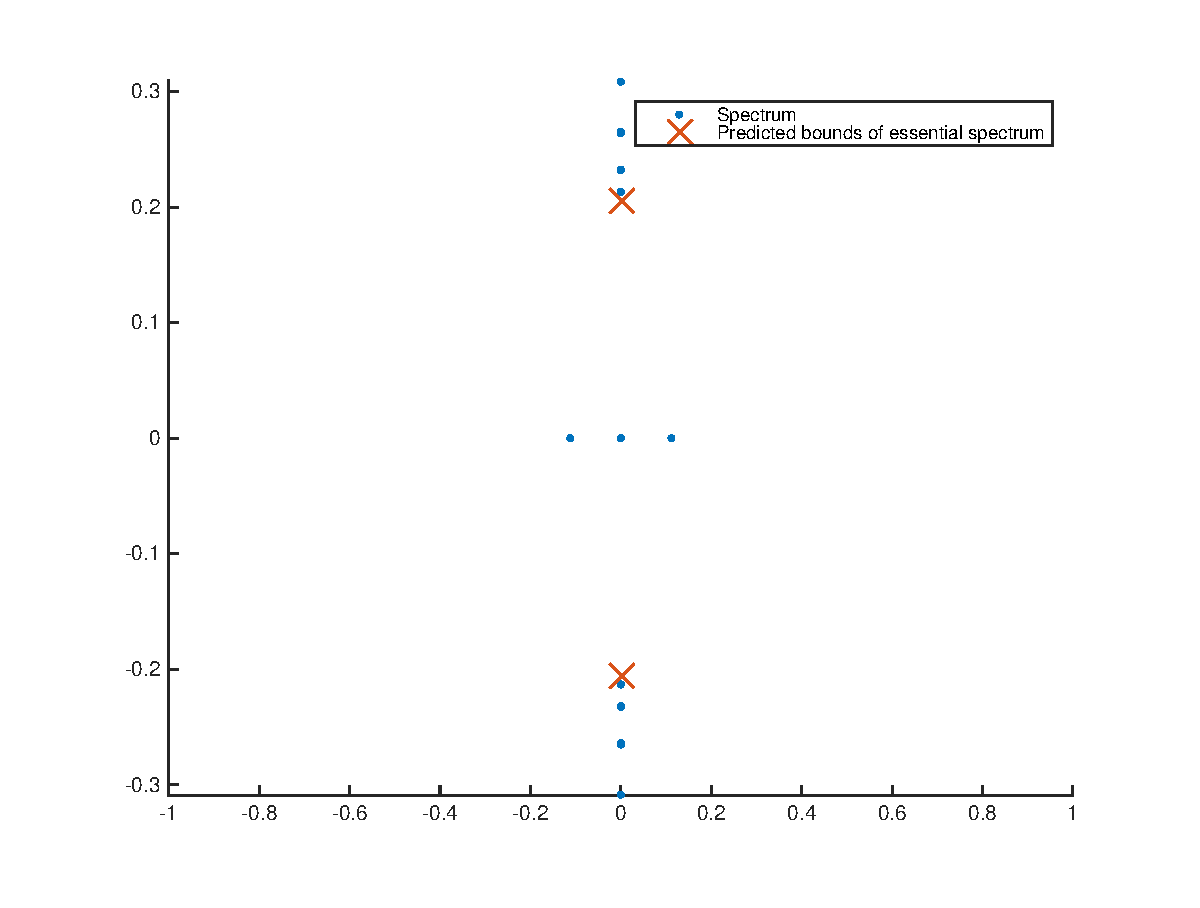
\includegraphics[width=8cm]{spec12_double1.eps}
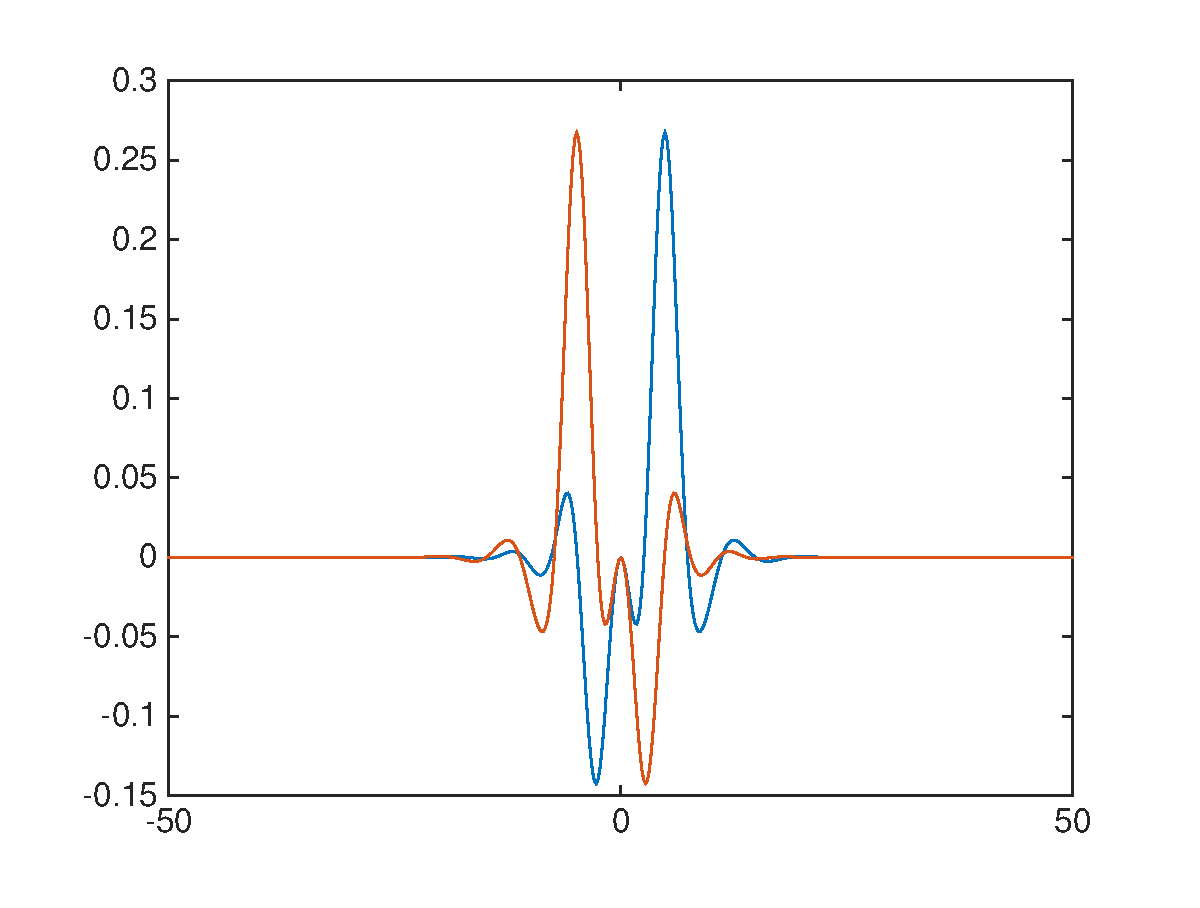
\includegraphics[width=8cm]{evecs12_double1.eps}
\caption{Linearization about Double Pulse 1. Spectrum (left) and interaction eigenfunctions (right). Finite difference methods, $N = 512$, $c = 1.2$.}
\end{figure}

Next we look at double pulse 2. Note that this time we have a pair of purely imaginary (to leading order; there is a small real part of order like 1e-10 just as with KdV5) eigenvalues. The plot below is only the real part of the eigenfunctions. It is easy to locate the interaction eigenvalues in this case, since we have bounds on the essential spectrum. The interaction eigenvalues lie inside the essential spectrum gap.

\begin{figure}[H]
\centering
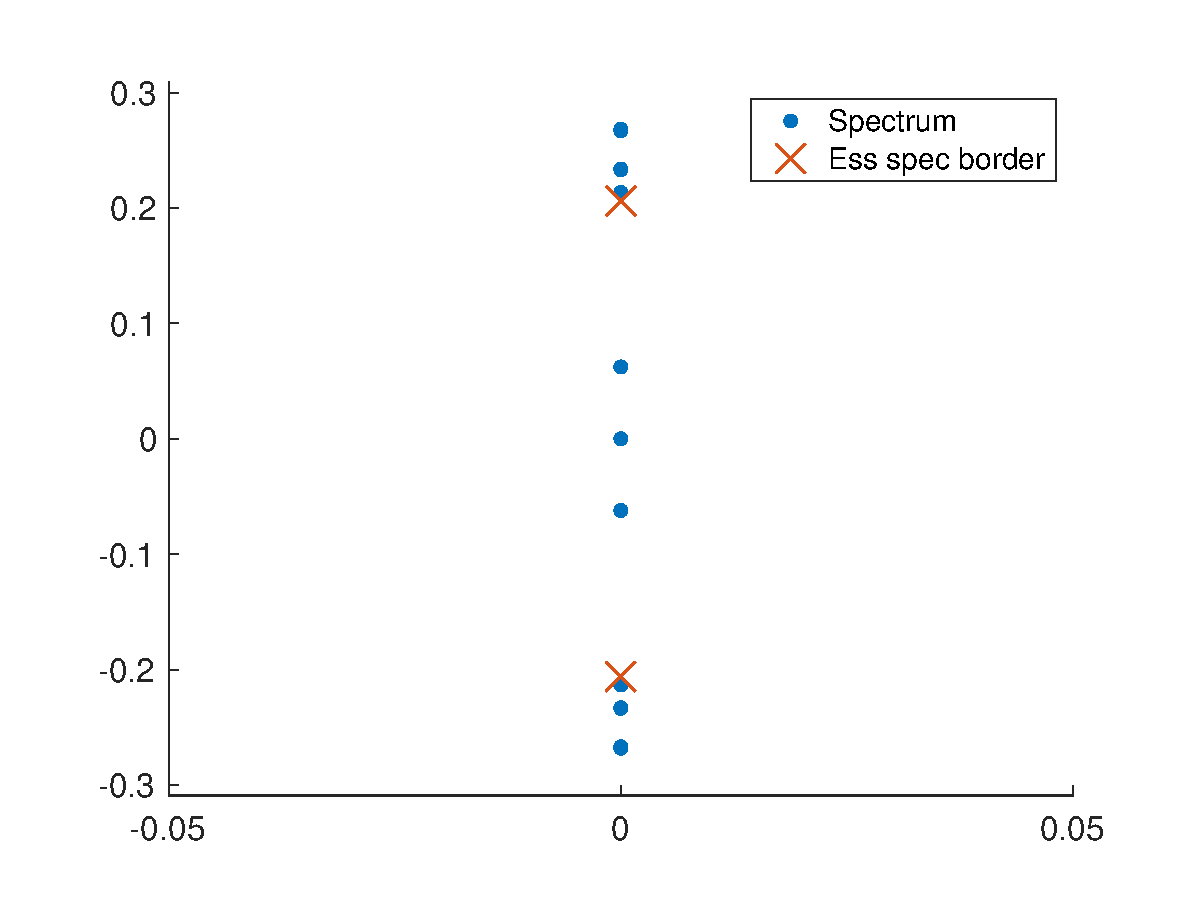
\includegraphics[width=8cm]{spec12_double2.eps}
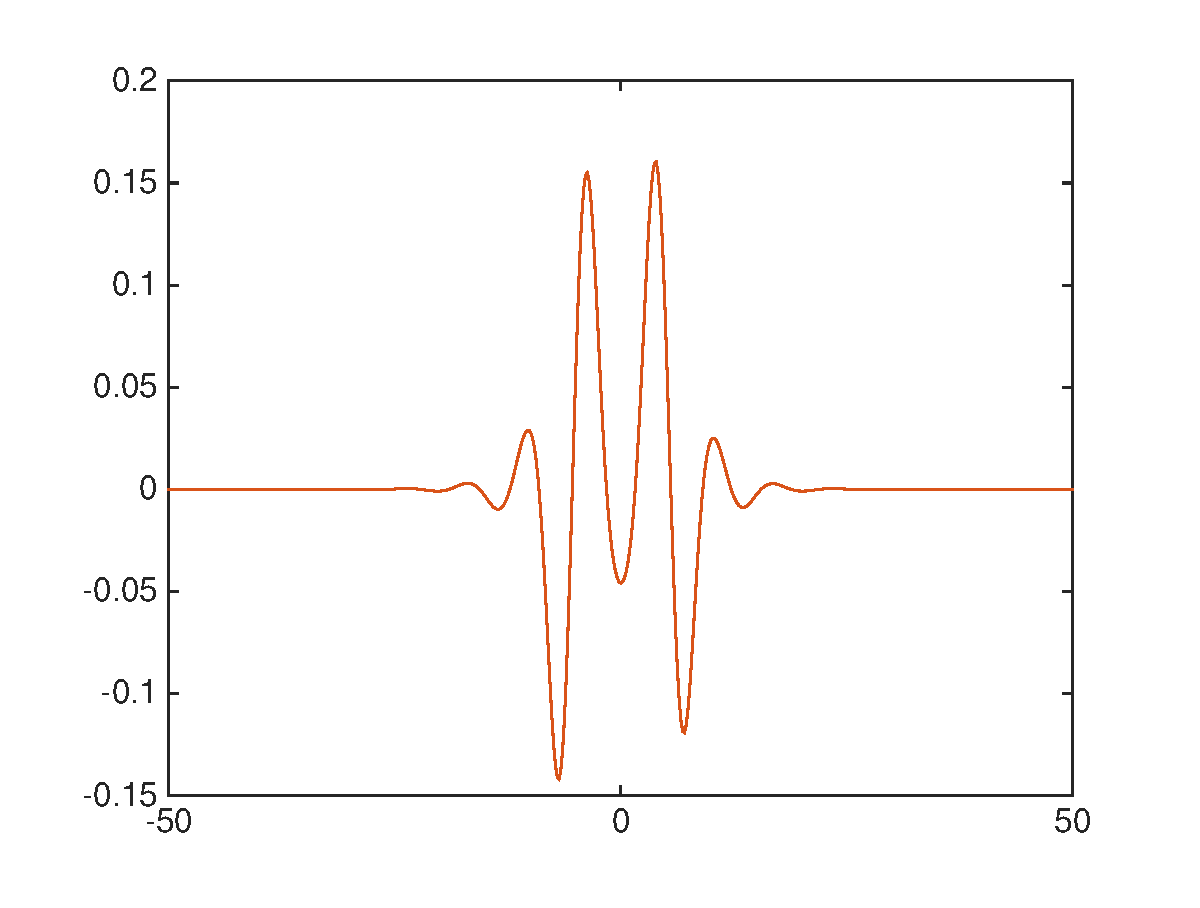
\includegraphics[width=8cm]{evecs12_double2real.eps}
\caption{Linearization about Double Pulse 2. Spectrum (left) and real part of interaction eigenfunctions (right). Finite difference methods, $N = 512$, $c = 1.2$.}
\end{figure}

The same pattern repeats (alternating pairs of real and purely imaginary interaction eigenvalues) as we go to higher double pulses.\\

We can also construct multipulses. For example, here is a triple pulse for $c = 1.2$ using the same pulse distance as double pulse 2. We get the expected two pairs of purely imaginary eigenvalues.

\begin{figure}[H]
\centering
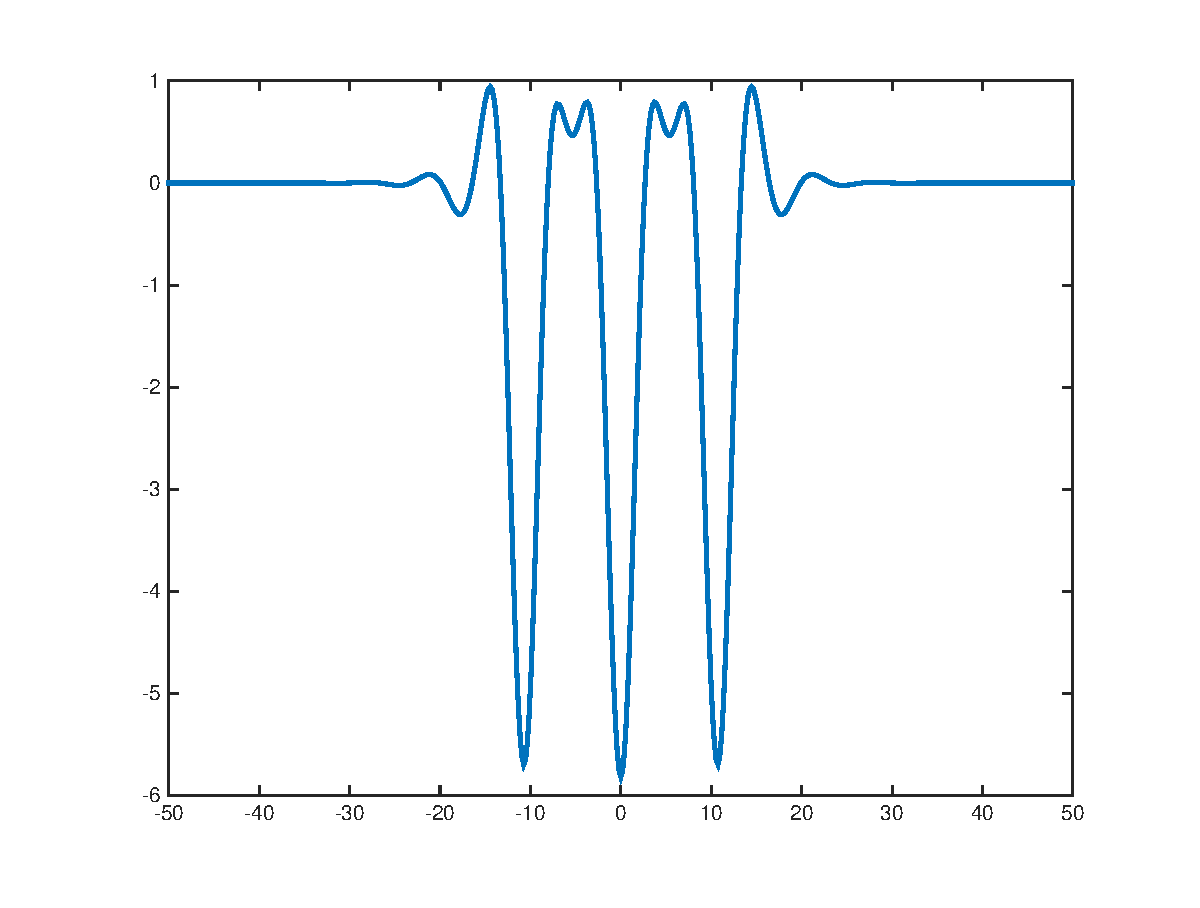
\includegraphics[width=8cm]{triple12_2.eps}
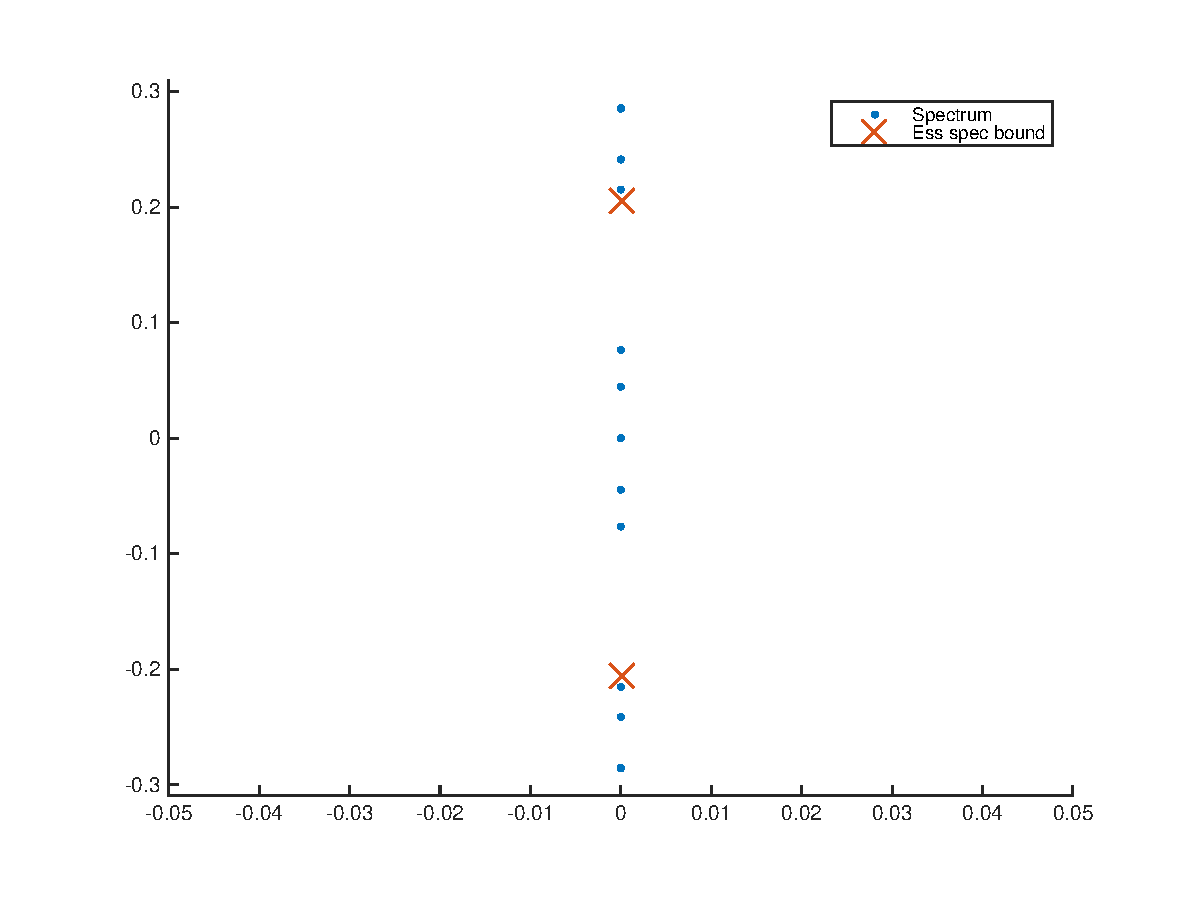
\includegraphics[width=8cm]{spec12_triple2.eps}
\caption{Triple pulse 2,2 (left). Spectrum of linearization about triple pulse 2,2 (right). Finite difference methods, $N = 512$, $c = 1.2$.}
\end{figure}

For other values of $c$, the odd-numbered double pulses have the same eigenvalue pattern, so we will focus on the even-numbered double pulses. Let's look at $c = 1.354$ (this value was used in \cite{Chen1997}). For Double Pulse 2, we now have a quartet of interaction eigenvalues. Their imaginary part now lies \emph{outside} the essential spectrum gap. This suggests that a Krein collision has occurred, where the interaction eigenvalues collide with the smallest essential spectrum eigenvalue and then form a quartet.

\begin{figure}[H]
\centering
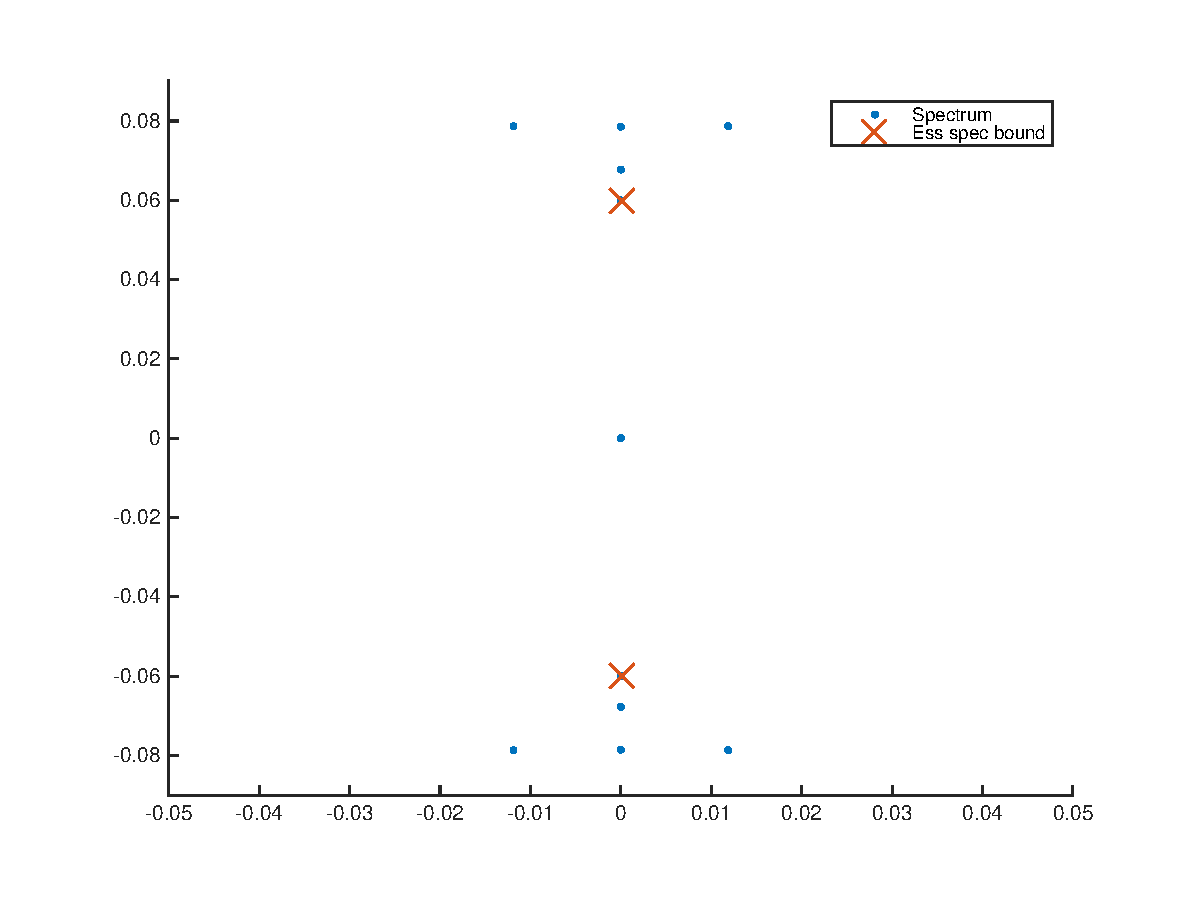
\includegraphics[width=8cm]{spec1354_double2.eps}
\caption{Linearization about Double Pulse 2. Spectrum showing Krein quartet. Finite difference methods, $N = 512$, $c = 1.354$.}
\end{figure}

The next two plots show that the Krein collision occurs between $c = 1.322$ (before collision) and $c = 1.323$ (after collision).

\begin{figure}[H]
\centering
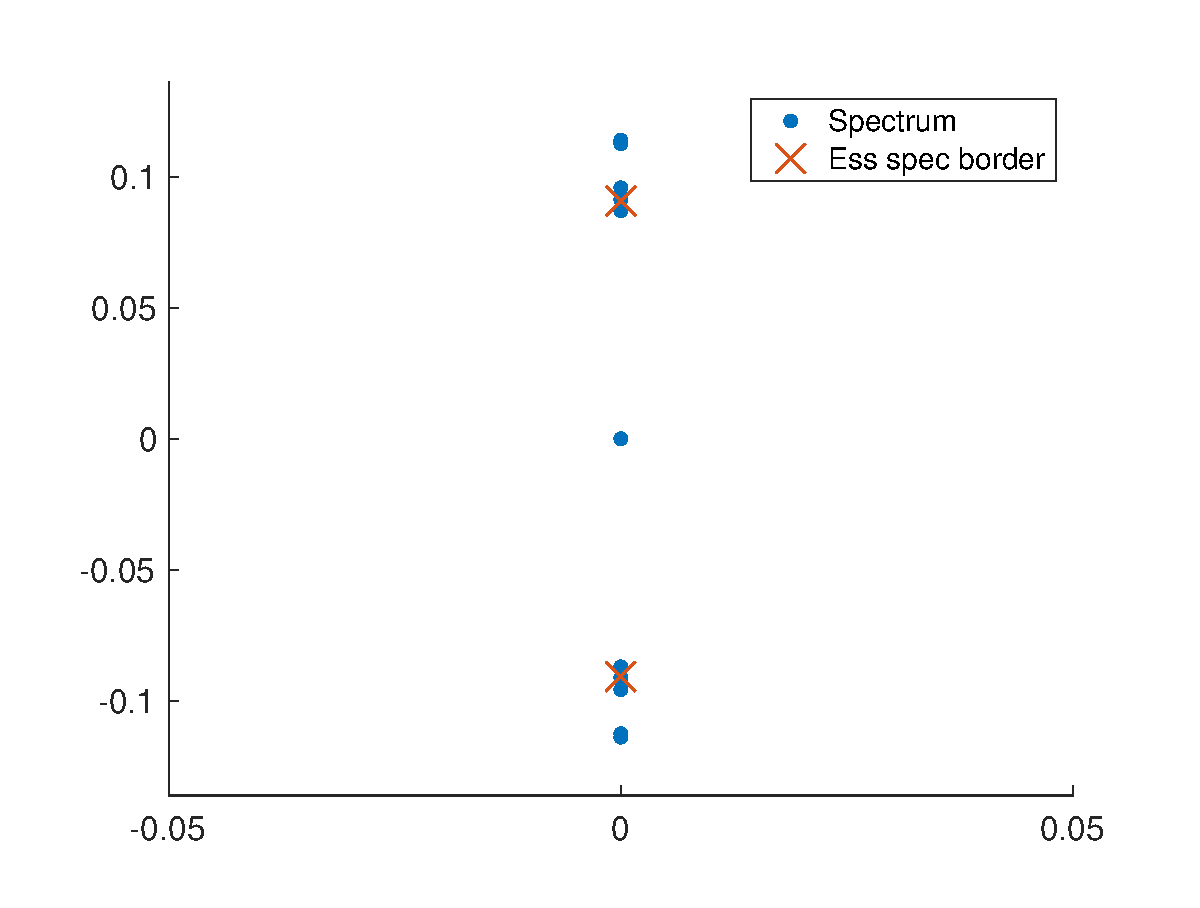
\includegraphics[width=8cm]{spec1322_double2.eps}
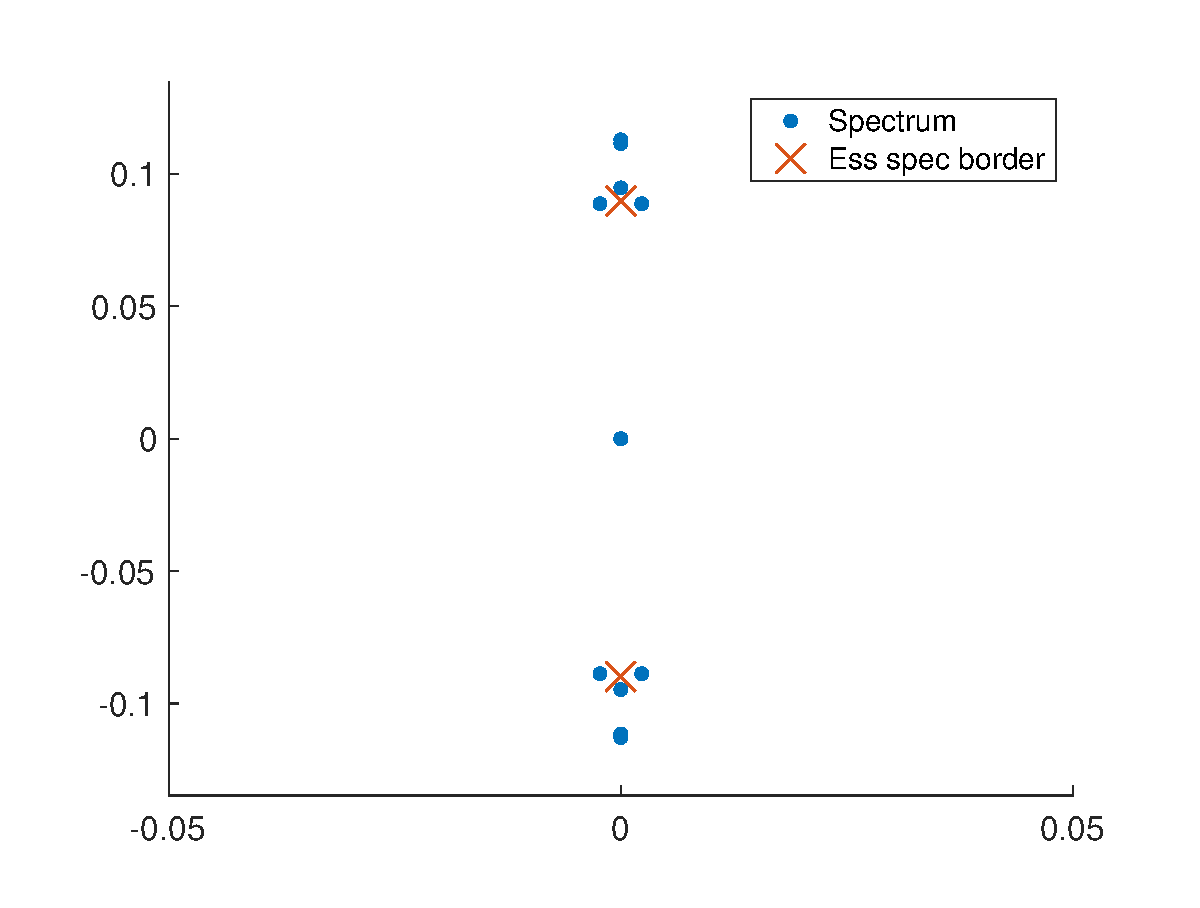
\includegraphics[width=8cm]{spec1323_double2.eps}
\caption{Linearization about Double Pulse 2. Spectrum before Krein collision ($c = 1.322$, left) and after Krein collision ($c = 1.323$, right). Finite difference methods, $N = 512$}
\end{figure}

\subsection{Krein Matrix}

\subsubsection{Background and Numerics}

We are finally ready to use the Krein matrix to compute the small eigenvalues of the quadratic eigenvalue problem \eqref{quadeig}.\\

Since $A_0(u_*)$ and $A_2$ are Hermitian and $A_1$ is skew-Hermitian, if we take $\lambda = i z$, where $z \in \R$, the quadratic operator $P_2(iz)$ is Hermitian.\\

Let $q_n$ be an $n-$pulse solution to \eqref{eqODE}, and let $S$ be the subspace spanned by the eigenfunctions of $A_0(q_n)$ corresponding to the $n$ eigenvalues near 0.

\begin{equation}\label{defS}
S = \spn\{s_1, \dots, s_n \}
\end{equation}

We found these eigenfunctions and eigenvalues in a previous section using Lin's method. Recall that $\nu_1 = 0$, the eigenfunctions are orthogonal, and that we have scaled the eigenfunctions so that 

\begin{equation}
\langle s_i, s_j \rangle = ||q_x||^2 \delta_{ij}
\end{equation}

where $q$ is the primary pulse.\\

First, we compute the Krein matrix numerically using the top of p.4 in Kap2018. As long as as choose $c$ small enough so that the Krein collision has not yet occurred, we get very accurate numerical results from this method (or at least they compare extremely well to the quadratic eigenvalue solver). 

\begin{table}[H]
\begin{tabular}{lll}
Pulse & From \texttt{quadeig} & imag part (from Krein Matrix) \\
Double Pulse 2    & $\pm 0.0622i$ & 0.0622 \\
Triple Pulse 2,2  & $\pm 0.0446i, \pm 0.0764i$ & 0.0446, 0.0764 \\
Double Pulse 2    & $\pm 0.0176i$ & 0.0176 \\
\end{tabular}
\caption{Eigenvalues from quadratic eigenvalue problem, computed with \texttt{quadeig} and from the Krein matrix. $c = 1.2$, finite difference method, $N = 512$. }
\end{table}

\subsubsection{Approximation for Small Eigenvalues}

To get analytical results, we use the approximation in Section 5 of Kap2018, since are are looking for eigenvalues near the origin. Recall that we take $\lambda = i z$, so the Krein matrix is a function of $z$. The operator $P_2(iz)$ is Hermitian, which implies that the Krein matrix is also Hermitian (p. 6 of Kap2018). In the case where we are looking for purely imaginary eigenvalues we have $z \in \R$.\\

Following Lemma 5.6 in Kap2018, for small $|z|$ the Krein matrix is the $n \times n$ matrix

\begin{equation}
K_S(z) = ||q_x||^2 \text{diag}(\nu_1, \dots, \nu_n) + \overline{z} K_1 - \overline{z}^2 \tilde{K}_2 + \mathcal{O}(|z|^3)
\end{equation}

where

\begin{equation}
(K_1)_{jk} = \langle s_j, i A_1 s_k \rangle
\end{equation}

and

\begin{equation}
(\tilde{K}_2)_{jk} = \langle s_j, (A_2 - A_1 P_{S^\perp} (P_{S^\perp} A_0(q_n) P_{S^\perp})^{-1} P_{S^\perp} A_1 ) s_k  \rangle
\end{equation}

Compared to Lemma 5.6, note that we have omitted the $-z$ out front, i.e. we use the form of the Krein matrix from p.4 rather than the form in Theorem 3.1. Since we also scaled the eigenfunctions differently, we have an additional factor of $||q_x||^2$ in the first term. The key observation is that this is, to leading order, a matrix-valued quadratic polynomial in $z$ (and its complex conjugate). In the case where we take $z$ to be real, this is a polynomial in $z$ only.\\

Since the operator $A_1$ is skew-Hermitian, $i A_1$ is Hermitian, thus for $K_1$ we have

\begin{align*}
(K_1)_{jk} = \langle s_j, i A_1 s_k \rangle &= \langle i A_1 s_j, s_k \rangle \\
&= \overline{ \langle s_k, i A_1 s_j \rangle } \\
&= \overline{ (K_1)_{kj} }
\end{align*}

As expected, $K_1$ is a Hermitian matrix. In particular, this implies that the diagonal entries are real. Since $A_0(q_n)$ and the eigenfunctions $s_i$ are real, $(K_1)_{ii} = \langle s_i, i A_1 s_i \rangle = \langle s_i, i A_1 s_i \rangle$ is purely imaginary, thus must be 0. We conclude that diagonal terms of $K_1$ are 0.\\

For the matrix $\tilde{K}_2$, we have 

\begin{align*}
(\tilde{K}_2)_{jk} &= \langle s_j, s_k \rangle - \langle s_j, A_1 P_{S^\perp} (P_{S^\perp} A_0(q_n) P_{S^\perp})^{-1} P_{S^\perp} A_1 s_k  \rangle \\
&= \langle s_j, s_k \rangle + \langle P_{S^\perp} A_1 s_j, (P_{S^\perp} A_0(q_n) P_{S^\perp})^{-1} P_{S^\perp} A_1 s_k  \rangle
\end{align*}

since $A_2 = I$. Since the eigenfunctions are orthogonal, by our chosen scaling we have, $\langle s_j, s_k \rangle = ||q_x||^2 \delta_{jk}$. Thus, $\tilde{K} = ||q_x||^2 I + K_2$, where

\begin{align*}
(K_2)_{jk} &= 
\langle P_{S^\perp} A_1 s_j, (P_{S^\perp} A_0(q_n) P_{S^\perp})^{-1} P_{S^\perp} A_1 s_k \rangle
\end{align*}

Since $A_0(q_n)$ and its spectral projections are self-adjoint, and $A_0(q_n)$ and the eigenfunctions are real, $K_2$ is a real, symmetric matrix. Thus the Krein matrix takes the form

\begin{equation}\label{Kreinform}
K_S(z) = ||q_x||^2 \text{diag}(\nu_1, \dots, \nu_n) + \overline{z} K_1 
- \overline{z}^2 ( ||q_x||^2 I + K_2) + \mathcal{O}(|z|^3)
\end{equation}

where $K_1$ and $K_2$ are defined above.\\

Next, we characterize the Krein matrix for the 1-pulse, since in that case will it will be a scalar.

% Lemma : Krein matrix, 1-pulse

\begin{lemma}\label{Krein1pulse}
For the linearization about the 1-pulse, the Krein matrix is the scalar

\begin{equation}
K(z) = d''(c) \overline{z}^2 + \mathcal{O}(z^3)
\end{equation}

where $d''(c)$ is the stability criterion from \cite{Grillakis1987}. The form of $d''(c)$ for this problem is given in \eqref{dcc}.

\begin{proof}

For the 1-pulse, there is exactly one eigenvalue at 0, for which the corresponding eigenfunction is $q_x$, i.e. $\nu_1 = 0$ and $s_1 = q_x$ (there is no scaling needed here). Let $S = \ker A_0(q)$ = $\spn \{q_x\}$. In this case, the Krein matrix will be 1x1, i.e. a scalar. Since $K_1$ is 0 on the diagonal, $K_1 = 0$. Thus we are left with

\begin{align*}
K(z) &= -\overline{z}^2 \left( ||q_x||^2 + \langle P_{S^\perp} A_1 q_x, (P_{S^\perp} A_0(q) P_{S^\perp})^{-1} P_{S^\perp} A_1 q_x \rangle \right) + \mathcal{O}(z^3) \\
&= -\overline{z}^2 \left( ||q_x||^2 + 4 c^2 \langle P_{S^\perp} q_{xx}, (P_{S^\perp} A_0(q) P_{S^\perp})^{-1} P_{S^\perp} q_{xx} \rangle \right) + \mathcal{O}(z^3)
\end{align*}

All that remains is to evaluate $P_{S^\perp} (P_{S^\perp} A_0(q) P_{S^\perp})^{-1} P_{S^\perp} q_{xx}$. Since $S$ is the span of a single odd function, and $q_{xx}$ is an even function, $P_{S^\perp} q_{xx} = q_{xx}$. Thus we only need to evaluate $(P_{S^\perp} A_0(q) P_{S^\perp})^{-1} q_{xx}$. Let $y = (P_{S^\perp} A_0(q) P_{S^\perp})^{-1} q_{xx}$. Then $(P_{S^\perp} A_0(q) P_{S^\perp})y = q_{xx}$. From \eqref{uc}, we have

\begin{equation*}\label{uc}
A_0(q) \left( -\frac{1}{2c} q_c \right) = q_{xx}
\end{equation*}

Thus $s = -(1/2c) q_c + k q_x$ for some scalar $k$. Substituting this into the equation for $K(z)$, and noting that the $k q_x$ term is wiped out by the projection $P_{S^\perp}$, we have

\[
K(z) = -\overline{z}^2 \left( ||q_x||^2 - 2c \langle q_{xx}, q_c \rangle \right) + \mathcal{O}(z^3)
\]

Integration by parts gives us

\begin{align*}
||q_x||^2 - 2c \langle q_{xx}, q_c \rangle &= \langle q_x, q_x \rangle + 2c \langle q_{x}, q_{xc} \rangle  \\
&= \langle q_x, q_x \rangle + c \frac{\partial}{\partial c}\langle q_x, q_x \rangle \\
&= ||q_x||^2 + c \frac{\partial}{\partial c}||q_x||^2 \\
&= \frac{\partial}{\partial c} \left( c||q_x||^2 \right)
\end{align*}

Thus the Krein matrix becomes 

\begin{align*}
K(z) &= -\frac{\partial}{\partial c} \left( c||q_x||^2 \right) \overline{z}^2 + \mathcal{O}(z^3) \\
&= d''(c) \overline{z}^2 + \mathcal{O}(z^3)
\end{align*}

\end{proof}
\end{lemma}

We will need the following result for exponentially localized functions, which we prove in the following lemma.

\begin{lemma}\label{exploc}
Let $q_+(x)$ and $q_-(x)$ be exponentially localized pulses which decay exponentially with rate $\alpha$ and whose peaks are separated by a distance $2 X$. Then 

\begin{enumerate}[(i)]
	\item $ || q_-(x) q_+(x)||_{L^\infty(\R)} \leq C e^{2 \alpha X}$ 
	\item $ | \langle q_-(x) q_+(x) \rangle | \leq C X e^{2 \alpha X}$ 
	\item For any $0 < \epsilon < \alpha$, $| \langle q_-(x) q_+(x) \rangle | \leq C e^{(2 \alpha - \epsilon) X}$ 
\end{enumerate}

\begin{proof}
Since we are working on $\R$ and the norms are translation invariant, we can WLOG take the peaks of $q_\pm(x)$ to be centered at $\pm X$, so that we have

\begin{align*}
|q_-(x)| \leq C e^{-\alpha|x + X|} \\
|q_+(x)| \leq C e^{-\alpha|x - X|} \\
\end{align*}

\begin{enumerate}[(i)]

\item For the $L^\infty$ norm, we split it up into four pieces and take the maximum over those pieces

\begin{align*}
|| q_-(x) & q_+(x)||_{L^\infty(\R)} \\
&= \max\{ || q_-(x) q_+(x)||_{L^\infty(-\infty, -X]} + || q_-(x) q_+(x)||_{L^\infty[-X, 0])} \\
&+ || q_-(x) q_+(x)||_{[0, X]} + || q_-(x) q_+(x)||_{L^\infty([X, \infty)} \}
\end{align*}

For $x \in (-\infty, -X]$ 

\begin{align*}
| q_-(x) q_+(x) | &\leq C e^{\alpha|x + X|} e^{-\alpha|x - X|} \\
&= C e^{\alpha(x + X)} e^{\alpha(x - X)} \\
&= C e^{2 \alpha x} \\
&\leq C e^{-2 \alpha X} 
\end{align*}

since we are on the interval $(-\infty, -X]$. For $x \in [-X,0]$, 

\begin{align*}
| q_-(x) q_+(x) | &\leq C e^{\alpha|x + X|} e^{-\alpha|x - X|} \\
&= C e^{-\alpha(x + X)} e^{\alpha(x - X)} \\
&= C e^{-2 \alpha X}  \\
\end{align*}

The other two pieces are similar, and give identical bounds. Since all four pieces have the same uniform bound, the result follows.

\item For the $L^2$ inner product, we again split the domain up into four pieces

\begin{align}\label{splitL2}
| \langle q_-(x) &q_+(x) \rangle | \\
&\leq \int_{-\infty}^{-X} |q_-(x) q_+(x)| dx + \int_{-X}^0 |q_-(x) q_+(x)|
+\int_0^X |q_-(x) q_+(x)| dx +\int_X^\infty |q_-(x) q_+(x)| dx \nonumber
\end{align}

For the first integral, we have

\begin{align*}
\int_{-\infty}^{-X} |q_-(x) q_+(x)| dx &\leq C \int_{-\infty}^{-X} e^{\alpha(x + X)} e^{\alpha(x - X)} dx \\
&= C \int_{-\infty}^{-X} e^{2 \alpha x} dx \\
&= C e^{-2 \alpha X}
\end{align*}

For the second integral, we have

\begin{align*}
\int_{-X}^0 |q_-(x) q_+(x)| dx &\leq C \int_{-X}^0 e^{-\alpha(x + X)} e^{\alpha(x - X)} dx \\
&= C \int_{-X}^0 e^{-2 \alpha X} dx \\
&= C X e^{-2 \alpha X}
\end{align*}

The other two integrals are similar. Combining these gives us the bound (ii). For the bound (iii), choose any $\epsilon$ with $0 < \epsilon < \alpha$. Then for the second integral in \eqref{splitL2}, we also have the bound

\begin{align*}
\int_{-X}^0 |q_-(x) q_+(x)| dx &\leq C \int_{-X}^0 e^{-\alpha(x + X)} e^{\alpha(x - X)} dx \\
&= C \int_{-X}^0 e^{-(\alpha-\epsilon)(x + X)} e^{-\epsilon(x + X)}  e^{\alpha x} e^{-\alpha X} dx \\ 
&= C e^{-(2 \alpha - \epsilon) X} \int_{-X}^0 e^{-(\alpha-\epsilon)x} e^{-\epsilon(x + X)}  e^{\alpha x}  dx \\ 
&= C e^{-(2 \alpha - \epsilon) X} \int_{-X}^0 e^{\epsilon x} e^{-\epsilon(x + X)} dx \\ 
&\leq C e^{-(2 \alpha - \epsilon) X} \int_{-X}^0 e^{-\epsilon(x + X)} dx \\ 
&= C e^{-(2 \alpha - \epsilon) X} \frac{1}{\epsilon}\left( 1 - e^{-\epsilon X} \right) dx \\ 
&\leq C e^{-(2 \alpha - \epsilon) X} dx \\ 
\end{align*}

where we used the fact that $0 < e^{\epsilon x} \leq 1$ since $x \leq 0$. Although we can choose any $\epsilon$ we want, the constant $C$ increases as $\epsilon$ gets smaller. The third integral in \eqref{splitL2} is similar. Since this bound is weaker than the bound for the first and fourth integrals in $\eqref{splitL2}$, the result (iii) follows.

\end{enumerate}

\end{proof}
\end{lemma}

In the next series of lemmas, we look at the individual components of the Krein matrix. First, we show that the matrix $K_1$ is exponentially small.

% lemma : K1 is exponentially small

\begin{lemma}\label{K1small}
The matrix $K_1$ is exponentially small, i.e. 

\begin{equation}
K_1 = \mathcal{O}(e^{-(3 \alpha/2) X_m} )
\end{equation}

\begin{proof}

Let $a_{jk} = (K_1)_{jk}$. We know from above that $a_{jj} = 0$, so we only need to consider the case $j \neq k$. Since $a_{jk} = \langle s_j, i A_1 s_k\rangle = 2 c i \langle s_j, (s_k)_x \rangle$, all we need to show is that $\langle s_j, (s_k)_x \rangle = \mathcal{O}(e^{-\alpha X_m})$. Using the expression \eqref{sj} for the eigenfunctions, we have

\begin{align*}
\langle s_j &, (s_k)_x \rangle = 
\langle \left( \sum_{i = 1}^{n} d_{ji} q^i_x + w_j \right) \left( \sum_{i = 1}^{n} d_{ki} q^j_{xx} + (w_k)_x \right) \rangle \\
&= \sum_{i = 1}^{n} d_{ji} d_{ki} \langle q^i_x, q^i_{xx} \rangle 
+ \sum_{i \neq l} d_{ji} d_{kl} \langle q^i_x, q^l_{xx} \rangle 
+ \langle \sum_{i = 1}^{n} d_{ji} q^i_x + w_j, (w_k)_x \rangle 
+ \langle w_j, \sum_{i = 1}^{n} d_{ki} q^j_{xx} \rangle \\
&= \sum_{i = 1}^{n} d_{ji} d_{ki} \langle q^i_x, q^i_{xx} \rangle 
+ \sum_{i \neq l} d_{ji} d_{kl} \langle q^i_x, q^l_{xx} \rangle 
+ \langle s_j, (w_k)_x \rangle 
+ \sum_{i = 1}^{n} d_{ki} \langle w_j, q^j_{xx} \rangle
\end{align*}  

For the first term on the RHS, since the $L^2$ inner product on $\R$ is translation invariant and the $q^i$ are translates of $q$, we have

\[
\langle q^i_x, q^i_{xx} \rangle = \langle q_x, q_{xx} \rangle = 0
\] 

since we are taking the inner product of an even and an odd function. For the second term on the RHS, we use Lemma \ref{exploc} with $\epsilon = \alpha / 2$. Since $q^i_x$ and $q^l_{xx}$ are exponentially separated by at least $2 X_m$, $\langle q^i_x, q^l_{xx} \rangle = \mathcal{O}(e^{-(3 \alpha/2) X_m})$. For the third term, by Holder's inequality,

\[
|\langle s_j, (w_k)_x \rangle| \leq ||s_j||_{L^1} ||(w_k)_x||_{L^\infty} \leq C e^{-2 \alpha X_m}
\]

using the remainder bound \eqref{sjwbound} and the fact that the eigenfunctions are exponentially localized, thus integrable. The same bound holds for the final term, again by Holder's inequality. Since the bound for the second term in the RHS is the weakest, it dictates the overall bound.

\end{proof}
\end{lemma}

Next, we show that the rows of the matrix $D$ defined in \eqref{matrixD} are orthonormal to leading order.

% lemma : orthogonal D

\begin{lemma}\label{orthogonalD}
Let $D$ be the matrix defined in \eqref{matrixD} representing the coefficients of the translates of the derivative of the primary pulse. Then the rows of $D$ are orthonormal to leading order, i.e. 

\begin{equation}
\sum_{i = 1}^{n} d_{ji} d_{ki} = \delta_{ij} + \mathcal{O}(e^{-(3 \alpha/2) X_m})
\end{equation}

\begin{proof}
Since the eigenvalues $\nu_i$ are distinct, the eigenfunctions $s_i$ are orthogonal. Recall that we have scaled them so that $||s_i|| = ||q_x||$. Thus, using the expression \eqref{sj} for the eigenfunctions, we have, similar to Lemma \ref{K1small}

\begin{align*}
||q_x||^2 \delta_{jk} &= \langle s_j, s_k \rangle \\
&= \langle \sum_{i = 1}^{n} d_{ji} q^i_x + w_j, \sum_{i = 1}^{n} d_{ki} q^i_x + w_k\rangle \\
&= \sum_{i = 1}^{n} d_{ji} d_{ki} \langle q^i_x, q^i_{x} \rangle 
+ \sum_{i \neq l} d_{ji} d_{kl} \langle q^i_x, q^l_{x} \rangle 
+ \langle s_j, w_k \rangle 
+ \sum_{i = 1}^{n} d_{ki} \langle w_j, q^j_{x} \rangle
\end{align*}

As in Lemma \ref{K1small}, the second term on the RHS is order $e^{-(3 \alpha/2) X_m}$ and the last two terms on the RHS are order $e^{-2 \alpha X_m}$. By translation invariance, we have for all $i$

\[
\langle q^i_x, q^i_{x} \rangle = \langle q_x, q_{x} \rangle = ||q_x||^2
\]

Thus we have
\[
||q_x||^2 \sum_{i = 1}^{n} d_{ji} d_{ki} = ||q_x||^2 \delta_{ij} + \mathcal{O}(e^{-(3 \alpha / 2) X_m})
\]

dividing by $||q_x||^2$ gives us
\[
\sum_{i = 1}^{n} d_{ji} d_{ki} = \delta_{ij} + \mathcal{O}(e^{-(3 \alpha / 2) X_m})
\]

\end{proof}
\end{lemma}

Before we can look at matrix $K_2$, we need to look at the term involving $(P_{S^\perp} A_0(q_n) P_{S^\perp})^{-1} P_{S^\perp} A_1 s_k$ which is found in $K_2$. We do that in a series of lemmas. First, we show that $(P_{S^\perp} A_0(q_n) P_{S^\perp})^{-1}$ is a bounded linear operator on $S^\perp$.

% lemma : PA_0 is invertible on Sperp

\begin{lemma}\label{PA0inv}
When restricted to $S^\perp$, $P_{S^\perp} A_0(q_n) |_{S^\perp}$ is an invertible linear operator, and its inverse $(P_{S^\perp} A_0(q_n)  |_{S^\perp})^{-1}$ is a bounded linear operator. If $z \in S^\perp$ is smooth, then $y = (P_{S^\perp} A_0(q_n)  |_{S^\perp})^{-1} z$ is smooth as well.

\begin{proof}
Consider the operator $P_{S^\perp} A_0(q_n) $. Since $A_0(q_n) $ is self-adjoint and the projection $P_{S^\perp}$ is self-adjoint, $P_{S^\perp} A_0(q_n) $ is also self-adjoint, since

\[
(P_{S^\perp} A_0(q_n) )^* = A_0(q_n) ^* P_{S^\perp}^* = A_0(q_n)  P_{S^\perp} = P_{S^\perp} A_0(q_n) 
\]

where the last equality holds since operators commute with their own spectral projections. We showed above that the essential spectrum of $A_0(q_n) $ is $\sigma_{\text{ess}} = [1, \infty)$. Thus for any $\lambda \notin [1, \infty)$, the operator $A_0(q_n)  - \lambda I$ is Fredholm with index 0. In particular, $A_0(q_n) $ and $(A_0(q_n)  - \nu_i I)$ are Fredholm with index 0. Since $A_0(q_n) $ is Fredholm, its range is closed. Thus by the closed range theorem (see Yosida, etc), 

\begin{equation}
\ran A_0(q_n)  = (\ker A_0(q_n)^*)^\perp = (\ker A_0(q_n))^\perp
\end{equation}

where the last equality holds since $A_0(q_n)$ is self-adjoint. Similarly, since $\nu \in \R$ and $\nu < 1$, we have

\begin{equation}\label{KerRangeNu}
\ran (A_0(q_n) - \nu_i I) = (\ker (A_0(q_n) - \nu_i I))^\perp 
\end{equation}

Next, we look at the kernel of $P_{S^\perp} A_0(q_n) = A_0(q_n) P_{S^\perp}$. This clearly contains $S$ (the kernel of $P_{S^\perp}$), but we need to ensure that it contains nothing else. It contains the kernel of $A_0(q_n)$, but $\ker A_0(q_n) = \spn\{ q_n' \}$, and $q_n' \in S$, so we have already taken care of that. Finally, it contains any function $y$ for which $(A_0(q_n) - \nu_i I) y = s_i$, since that will be wiped out by the projection $P_{S^\perp}$. But we cannot have a function $y$ with $(A_0(q_n) - \nu_i I) y = s_i$, since by \eqref{KerRangeNu}, we would have $s_i \perp \ker (A_0(q_n) - \nu_i I)$, which contains $s_i$. Thus we conclude that

\[
\ker P_{S^\perp} A_0(q_n) = S 
\]

Since the range of $A_0(q_n)$ is closed and $P_{S^\perp}$ is bounded, the range of $P_{S^\perp} A_0(q_n)$ is closed. Thus by the closed range theorem and the fact that $P_{S^\perp} A_0(q_n)$ is self-adjoint,

\[
\ran P_{S^\perp} A_0(q_n) = (\ker (P_{S^\perp} A_0(q_n))^*)^\perp = (\ker (P_{S^\perp} A_0(q_n)))^\perp = S^\perp
\]

Since $\dim \ker P_{S^\perp} A_0(q_n) = \text{codim } P_{S^\perp} A_0(q_n) = 2$, $P_{S^\perp} A_0(q_n)$ is a Fredholm operator with index 0.\\

If we restrict the operator $P_{S^\perp} A_0(q_n)$ to $S^\perp$ (which is well-defined since its range is $S^\perp$), we get rid of the 2-dimensional kernel, thus obtain an invertible operator. Thus for $z \in S^\perp$ we can solve the equation

\[
(P_{S^\perp} A_0(q_n)) y = z
\]

uniquely for $y \in S^\perp$, i.e. we have for $z \in S^\perp$,

\begin{equation}
y = (P_{S^\perp} A_0(q_n) |_{S^\perp})^{-1} z
\end{equation}

Note that in Kap2018, this operator is written $(P_{S^\perp} A_0(q_n) P_{S^\perp})^{-1}$. Since the spectrum of $P_{S^\perp} A_0(q_n) |_{S^\perp}$ is bounded away from 0 (by what we discussed above about the spectrum of $A_0(q_n)$), the spectrum of $(P_{S^\perp} A_0(q_n) |_{S^\perp})^{-1}$ is bounded by a constant, i.e. 

\[
\text{spec } P_{S^\perp} A_0(q_n) |_{S^\perp}  \subset [-\rho, \rho]
\]

for some $\rho > 0$. Since $P_{S^\perp} A_0(q_n)$ is self-adjoint, we can use the resolvent bound for normal operators to conclude that $(P_{S^\perp} A_0(q_n) |_{S^\perp})^{-1}$ is a bounded linear operator with operator norm

\[
|| (P_{S^\perp} A_0(q_n)|_{S^\perp})^{-1} || \leq \frac{1}{\rho}
\]

Since $A_0(q_n): H^4 \in L^2 \rightarrow L^2$, if $z$ is smooth then $y (P_{S^\perp} A_0(q_n) |_{S^\perp})^{-1} z$ must be smooth as well.

\end{proof}
\end{lemma}

Next, using the definition for $A_1$ and the expression \eqref{sj} for $s_k$, we need to evaluate

\begin{align*}
(P_{S^\perp} A_0(q_n) P_{S^\perp})^{-1} P_{S^\perp} A_1 s_k 
&= -2c \sum_{i = 1}^{n} d_{ji} (P_{S^\perp} A_0(q_n) P_{S^\perp})^{-1} P_{S^\perp} q^i_{xx} + (P_{S^\perp} A_0(q_n) P_{S^\perp})^{-1} P_{S^\perp} (w_j)_x 
\end{align*}

Since $(P_{S^\perp} A_0(q_n) P_{S^\perp})^{-1}$ is a bounded linear operator and the remainder term $(w_j)_x = \mathcal{O}(e^{-\alpha X_m})$, the last term on the RHS is also $\mathcal{O}(e^{-\alpha X_m})$. Thus all we need to do is evaluate $(P_{S^\perp} A_0(q_n) P_{S^\perp})^{-1} P_{S^\perp} q^i_{xx}$. We will do this using Lin's method. Before we can do that, we prove a useful lemma and corollary which gives a leading order expansion for $e^{q_n(x)}$.

% lemma : exponential separation 

\begin{lemma}\label{expsep}

For the $n-$pulse $q_n(x)$ and for all $i = 1, \dots, n$

\begin{equation}
\exp(q_n(x)) = \exp( q^i(x)) + \sum_{j \neq i} (\exp(q^j(x)) - 1) + \mathcal{O}(e^{-\alpha X_m}) 
\end{equation}

\begin{proof}

Recall from \eqref{qn} that 

\[
q_n = \sum_{i = 1}^{n} q^i + \mathcal{O}(e^{-\alpha X_m})
\]

Fix $i$, and let $s(x) = \sum_{j \neq i} q_j(x)$. Then we have

\[
q_n = q^i + s + \mathcal{O}(e^{-\alpha X_m})
\]

Using a Taylor expansion, 

\begin{align*}
\exp(q_n(x)) &= \exp( q^i(x) + s(x) + \mathcal{O}(e^{-\alpha X_m}) ) \\
&= \exp( q^i(x) + s(x) ) \exp( \mathcal{O}(e^{-\alpha X_m}) )\\
&= \exp( q^i(x) + s(x) ) (1 + \mathcal{O}(e^{-\alpha X_m})) \\
&= \exp( q^i(x) + s(x) ) + \mathcal{O}(e^{-\alpha X_m}) \\
&= \exp( q^i(x) )\exp(s(x)) + \mathcal{O}(e^{-\alpha X_m})
\end{align*}

where the penultimate line holds since $q$ is bounded. Looking at the first term on the RHS, we have

\begin{align*}
\exp( q^i(x))\exp(s(x)) &=
\sum_{m=0}^\infty \frac{q^i(x)^m}{m!}
\sum_{n=0}^\infty \frac{s(x)^n}{n!}\\
&= \sum_{m=0}^\infty \frac{q^i(x)^m}{m!} 
+ \sum_{n=0}^\infty\frac{s(x)^n}{n!} - 1 +
\sum_{m=1}^\infty \frac{q^i(x)^m}{m!}
\sum_{n=1}^\infty \frac{s(x)^n}{n!} \\
&= \exp( q^i(x)) + \exp(s(x)) - 1 +
q^i(x)s(x)\sum_{m=0}^\infty \frac{q^i(x)^m}{(m+1)!}
\sum_{n=0}^\infty \frac{s(x)^n}{(n+1)!}
\end{align*}

For the final term on the RHS, we have

\begin{align*}
\left| q^i(x)s(x)\sum_{m=0}^\infty \frac{q^i(x)^m}{(m+1)!} \sum_{n=0}^\infty \frac{s(x)^n}{(n+1)!} \right| 
&\leq \left| q^i(x)s(x) \right| \sum_{m=0}^\infty \frac{|q^i(x)|^m}{m!} 
\sum_{n=0}^\infty \frac{|s(x)|^n}{n!} \\
&\leq \left| q^i(x)s(x) \right| e^{|q^i(x)|}e^{|s(x)|} \\
&\leq C \left| q^i(x)s(x) \right|
\end{align*}

where in the last line we used the fact that $q$ is bounded. Since all $n$ peaks are exponentially separated, so are $q^i(x)$ and $s(x)$, thus from Lemma \ref{expsep}, $\left| q^i(x)s(x) \right| = \mathcal{O}(e^{-\alpha 2 X_m})$. Putting this all together, we have

\begin{equation}
\exp(q_n) = \exp( q^i(x)) + (\exp(s(x)) - 1) + \mathcal{O}(e^{-\alpha X_m}) 
\end{equation}

Repeat this $n - 2$ more times to get the result.

\end{proof}
\end{lemma}

With this taken care of, we will use Lin's method to solve $(P_{S^\perp} A_0(q_n) |_{S^\perp})^{-1} P_{S^\perp} q^i_{xx}$.

% lemma : solve with Lin's method

\begin{lemma}\label{Linsolve}
For all $i = 1, \dots, n$,
 
\begin{equation}
(P_{S^\perp} A_0(q_n)|_{S^\perp})^{-1} P_{S^\perp} q^i_{xx} = -\frac{1}{2c}P_{S^\perp} q^i_c
+ \tilde{w}_i
\end{equation}

where $\tilde{w}_i$ is smooth and 

\begin{equation}
||\tilde{w}_i|| = \mathcal{O}(e^{-2 \alpha X_m})
\end{equation}

\begin{proof}
For convenience, let $k = -1/2c$, so that $A_0(q) k q_c$ = $q_{xx}$. Since everything involved is translation invariant, we also have $A_0(q^i) k q^i_c$ = $q^i_{xx}$. Applying the projection $P_{S^\perp}$ on both sides and using the fact that $A_0(q_n)$ commutes with its own spectral projections, we have

\begin{align*}
P_{S^\perp} A_0(q_n) k q^i_c &= P_{S^\perp} q^-_{xx} \\
A_0(q_n) (P_{S^\perp} k q^i_c) &= P_{S^\perp} q^i_{xx}
\end{align*}

Using this as motivation, we will look for a solution $y$ to 

\begin{equation}\label{Lineq1}
(P_{S^\perp} A_0(q_n)) y = P_{S^\perp} q^i_{xx}
\end{equation}

of the form

\begin{equation}\label{yansatz}
y = P_{S^\perp} k q^i_c + \tilde{w}
\end{equation}

We will use Lin's method to show that $\tilde{w}$ is exponentially small. Using Lemma \ref{expsep}, for $i = 1, \dots, n$ we can write $A_0(q_n)$ as 

\begin{align}\label{A0expansion} 
A_0(q_n) &= \partial_x^4 + c^2 \partial_x^2 + e^{q^i(x)} + \sum_{j \neq i} (e^{q^j(x)} - 1) + \tilde{h}(x) \\
&= A_0(q^i) + \sum_{j \neq i} (e^{q^j(x)} - 1) + \tilde{h}(x) \nonumber
\end{align}

where $||\tilde{h}|| = \mathcal{O}(e^{-\alpha X}$. Substituting in our ansatz \eqref{yansatz} for $y$ in \eqref{Lineq1}, we obtain

\begin{align*}
A_0(q_n) (P_{S^\perp} k q^i_c + \tilde{w}) &= P_{S^\perp} q^i_{xx} \\
\left(\partial_x^4 + c^2 \partial_x^2 + e^{q^i(x)} + \sum_{j \neq i} (e^{q^j(x)} - 1) + \tilde{h}(x) \right)P_{S^\perp} k q^i_c + A_0(q_n) \tilde{w} &= P_{S^\perp} q^i_{xx} \\
(\partial_x^4 + c^2 \partial_x^2 + e^{q^i(x)})P_{S^\perp} k q^i_c + \left( \sum_{j \neq i} (e^{q^j(x)} - 1)+ \tilde{h}(x) \right) P_{S^\perp}k q^i_c + A_0(q_n) \tilde{w} &= P_{S^\perp} q^i_{xx} \\
A_0(q_n) \tilde{w} + \underbrace{\left( \sum_{j \neq i} (e^{q^j(x)} - 1)\right) P_{S^\perp} k q^i_c}_{\mathcal{O}(e^{-\alpha X})} 
+ \underbrace{h(x) P_{S^\perp}k q^i_c}_{\mathcal{O}(e^{-\alpha X})} &= 0 \\
A_0(q_n) \tilde{w} + h(x) &= 0
\end{align*}

where we have collected all of the $\mathcal{O}(e^{-\alpha X})$ stuff and called it $h(x)$. Note that $A_0(q_n)$ is still the linearization about the $n$-pulse, but we will separate that out in the next step using our expansion \eqref{A0expansion} for $A_0(q_n)$.\\

Next, following \cite{Sandstede1998}, we write this piecewise as a first order system. For convenience of notation, we use the notation $W$ when we write $\tilde{w}$ in the first order system. First, as in \cite{Sandstede1998}, we choose the $2n$ intervals 

\begin{align*}
(-\infty, 0], [0, X_1], [-X_1, 0], [0, X_2], \dots, [-X_{n-1}, 0], [0, \infty)
\end{align*}

Then, using the expansions \eqref{A0expansion} for $A_0(q_n)$ (and noting the shift of coordinates), we obtain the first order system

\begin{align*}
(W_i^\pm)'(x) = A(q(x)) W_i^\pm(x) + G_i(x) W_i^\pm(x) + B H(x)
\end{align*}

where

\begin{align*}
A(q(x)) &= \begin{pmatrix}
0 & 1 & 0 & 0 \\
0 & 0 & 1 & 0 \\
0 & 0 & 0 & 1 \\
-e^{q(x)} & 0 & -c^2 & 0 
\end{pmatrix},
B = \begin{pmatrix}
0 & 0 & 0 & 0 \\
0 & 0 & 0 & 0 \\
0 & 0 & 0 & 0 \\
1 & 0 & 0 & 0 
\end{pmatrix},
G_i(x) &= \begin{pmatrix}
0 & 0 & 0 & 0 \\
0 & 0 & 0 & 0 \\
0 & 0 & 0 & 0 \\
\sum_{j \neq i} (1 - e^{q(x - \rho_{ji})}) & 0 & 0 & 0 
\end{pmatrix}
\end{align*}

The key here is that the expansions for $A_0(q_n)$ in \eqref{A0expansion} depend on $i$, so we have a different expansion on each piece. Now we use Lin's method, i.e. look to solve the equations

\begin{align}
(W_i^\pm)'(x) &= A(q(x)) W_i^\pm(x) + G_i(x) W_i^\pm(x)+ B H(x) \nonumber \\
W_1^+(X) - W_2^-(-X) &= 0 \label{Wsystem} \\
W_i^-(0) - W_i^+(0) \in \C \Psi(0) \nonumber 
\end{align}

Where $\Psi(x)$ is the unique bounded solution to the adjoint equation $W' = -A(q(x))^* W$. These equations, solved via Lin's method, will give us a unique solution $W_i^\pm$, but in general these will have jumps $n$ at $x = 0$ (in the piecewise coordinate system).\\

From the bound on $h$, we have $||H|| = \mathcal{O}(e^{-\alpha X_m)}$. On the $i^\pm$ pieces, we note that by construction $q(x - \rho_{ji}) = \mathcal{O}(e^{-\alpha X_m})$ on the interval $[-X_{i-1}, X_i]$. Thus, using a Taylor series, we have on that interval

\begin{align*}
1 - e^{q(x - \rho_{ji})} &= q(x - \rho_{ji}) + \mathcal{O}(q(x - \rho_{ji}))^2 = \mathcal{O}(e^{-\alpha X_m})
\end{align*}

We conclude that $||G|| = \mathcal{O}(e^{-\alpha X_m)}$. With these bounds, we are set up to use Lin's method. Following \cite{Sandstede1998} (or another suitable reference), we obtain unique functions $W_i^\pm$ which solve \eqref{Wsystem}. In adapting \cite{Sandstede1998}, we note that our system is similar to (3.7) in \cite{Sandstede1998}, except the $d_i$ is missing (we take it to be 1), there is no $\lambda$ (we take it to be 1), $D = 0$, and the $\lambda B_i^\pm$ term is absent entirely. The jumps are given by Lemma 3.6 in \cite{Sandstede1998}.

\begin{equation}
\xi_i = \int_{-\infty}^\infty \langle \Psi(x), H(x) \rangle dx + R_i
\end{equation}

where the $R_i$ are remainder terms for which $R = \mathcal{O}(e^{-3 \alpha X_m})$. A uniform bound on $W_i^\pm$ comes from Lin's method and is given by 

\begin{equation}\label{Wbound}
||W|| \leq C e^{-2 \alpha X_m}
\end{equation}

Taking this out of the first order system form, we have constructed via Lin's method a piecewise solution $y_i^\pm = P_{S^\perp} k q^i+_c + \tilde{w}_i^\pm$ to the problem $A_0(q_n) y = P_{S^\perp} q^i_{xx}$. What we want is solution $y \in \ran P_{S^\perp}$ to $P_{S^\perp} A_0(q_n) y = P_{S^\perp} q^i_{xx}$, i.e. we want the operator $P_{S^\perp} A_0(q_n)$ instead $A_0(q_n)$. But we can easily get this by applying the projection $P_{S^\perp}$ to both sides.

\begin{align*}
P_{S^\perp} A_0(q_n) y_i^\pm &= P_{S^\perp} P_{S^\perp} q^i_{xx} \\
P_{S^\perp} P_{S^\perp} A_0(q_n) y_i^\pm &= P_{S^\perp} q^i_{xx} \\
P_{S^\perp} A_0(q_n) (P_{S^\perp} y_i^\pm) &= P_{S^\perp} q^i_{xx}
\end{align*}

where we used the fact that $P_{S^\perp}$ is a spectral projection and thus commutes with $A_0(q_n)$. Thus $P_{S^\perp} y_i^\pm \in \ran P_{S^\perp}$ and $P_{S^\perp} A_0(q_n) (P_{S^\perp} y_i^\pm) = P_{S^\perp} q^i_{xx}$. Since everything above is in $S^\perp$, this is equivalent to

\begin{equation}
(P_{S^\perp} A_0(q_n))|_{S^\perp} (P_{S^\perp} y_i^\pm) = P_{S^\perp} q^i_{xx}
\end{equation}

We showed in Lemma \ref{PA0inv} that $(P_{S^\perp} A_0(q_n))|_{S^\perp}$ is an invertible operator on $S^\perp$. Thus $y = (P_{S^\perp} A_0(q_n))|_{S^\perp} P_{S^\perp} q^i_{xx}$ is the unique solution to the problem $P_{S^\perp} A_0(q_n) = P_{S^\perp} q^i_{xx}$. Since $P_{S^\perp} y_i^\pm$ is another such solution, they must be identical. In particular, from Lemma \ref{PA0inv}, since $P_{S^\perp} q^i_{xx}$ is smooth, $y$ must be smooth as well. Since $P_{S^\perp} k q^+_c$ is smooth and $y = P_{S^\perp} k q^i_c + P_{S^\perp} \tilde{w}_i^\pm$, $P_{S^\perp} \tilde{w}_i^\pm$ must be smooth. In particular, this implies that the jumps $\xi_i$ are all 0. Since projections are bounded with norm of 1, using the uniform bound \eqref{Wbound} on $||W||$ we have 

\[
P_{S^\perp} \tilde{w}_i^\pm = \mathcal{O}(e^{-2 \alpha X_m})
\]

Thus the unique solution in $S^\perp$ to $P_{S^\perp} A_0(q_n) y = P_{S^\perp} q^i_{xx}$.

\begin{align*}
y &= P_{S^\perp} k q^i_c + \tilde{w}_i
\end{align*}

where

\begin{align*}
||\tilde{w}_i|| = \mathcal{O}e^{-2 \alpha X_m}
\end{align*}

\end{proof}
\end{lemma}

Finally, we show that the matrix $K_2$ is diagonally dominant

% lemma : K_2 is diagonally dominant

\begin{lemma}\label{K2exp}

The matrix $K_2$ is given, to leading order, by

\begin{equation}
K_2 = -2c \langle q_{xx}, q_c \rangle I + \mathcal{O}(e^{-(3 \alpha/2) X_m})
\end{equation}

\begin{proof}

\begin{align*}
(K_2)_{jk} 
&= 4 c^2 \langle P_{S^\perp} (s_j)_{x}, (P_{S^\perp} A_0(q_n) P_{S^\perp})^{-1} P_{S^\perp} (s_k)_{x} \rangle \\
&= 4 c^2 \langle (s_j)_{x}, P_{S^\perp}(P_{S^\perp} A_0(q_n) P_{S^\perp})^{-1} P_{S^\perp} (s_k)_{x} \rangle \\
&= 4 c^2 \langle \sum_{i = 1}^{n} d_{ji} q^i_{xx} + (w_j)_x, P_{S^\perp} (P_{S^\perp} A_0(q_n) P_{S^\perp})^{-1} P_{S^\perp} \left( \sum_{i = 1}^{n} d_{ki} q^i_{xx} + (w_k)_x \right) \rangle \\
&= -\frac{1}{2 c} 4 c^2 
\langle \sum_{i = 1}^{n} d_{ji} q^i_{xx} + (w_j)_x, \sum_{i = 1}^{n} d_{ki} q^i_c + \mathcal{O}(e^{-2 \alpha X_m}) \rangle \\
\end{align*}

where we used Lemma \ref{Linsolve}, the fact that $(P_{S^\perp} A_0(q_n) P_{S^\perp})^{-1}$ is a bounded linear operator from Lemma \ref{PA0inv}, and the bound on the remainder terms $w_i$ from Lemma \ref{Linsolve}. Simplifying this, we have

\begin{align*}
(K_2)_{jk} &= -2 c \left( 
\langle \sum_{i = 1}^{n} d_{ji} q^i_{xx} + (w_j)_x, \sum_{i = 1}^{n} d_{ki} q^i_c + \mathcal{O}(e^{-2 \alpha X_m}) \rangle \right) \\
&= -2 c \left( \sum_{i = 1}^{n} d_{ji} d_{ki} \langle q^i_{xx}, q^i_c \rangle
+ \sum_{i\neq l} d_{ji} d_{kl} \langle q^i_{xx}, q^j_c \rangle
+ \langle (s_j)_x,  \mathcal{O}(e^{-2 \alpha X_m}) \rangle 
+ \sum_{i=1}^n \langle (w_j)_x, d_{ki} q^i_c \rangle \right)
\end{align*}

Since $q^i_{xx}$ and $q^j_c$ are exponentially separated for $i \neq j$ by at least $X_m$, the second term on the RHS is $\mathcal{O}(e^{-(3 \alpha/2) X_m})$ as in Lemma \ref{K1small}. The last two terms on the RHS are $\mathcal{O}(e^{-\alpha X_m})$ as in Lemma \ref{K1small}. The first term on the RHS is

\begin{align*}
\sum_{i = 1}^{n} d_{ji} d_{ki} \langle q^i_{xx}, q^i_c \rangle &= \sum_{i = 1}^{n} d_{ji} d_{ki} \langle q_{xx}, q_c \rangle \\
&= \langle q_{xx}, q_c \rangle \sum_{i = 1}^{n} d_{ji} d_{ki} \\
&= \langle q_{xx}, q_c \rangle \delta_{jk} + \mathcal{O}(e^{-(3 \alpha/2) X_m})
\end{align*}

where the sum is given by Lemma \ref{orthogonalD}. Thus we have

\begin{align*}
K_2 = -2c \langle q_{xx}, q_c \rangle + \mathcal{O}(e^{-(3\alpha /2)X_m})
\end{align*}

\end{proof}
\end{lemma}

We combine these lemmas in the following theorem

\begin{theorem}\label{Kreindiagdom}
For the linearization of the suspension bridge equation about an $n-$pulse equilibrium solution $q_n(x)$, the Krein matrix is given by

\begin{equation}\label{Kreinapprox}
K_S(z) = ||q_x||^2 \text{diag}(\nu_1, \dots, \nu_n)
 + d''(c) I \overline{z}^2 + \mathcal{O}(e^{-(3 \alpha/2) X_m}|z| + |z|^3)
\end{equation}

\begin{proof}

From \eqref{Kreinform}, Lemma \ref{K1small} and Lemma \ref{K2exp}, we have

\begin{align*}
K_S(z) &= ||q_x||^2 \text{diag}(\nu_1, \dots, \nu_n) + \overline{z} \mathcal{O} (e^{-(3 \alpha/2) X_m})
 - \overline{z}^2 ( (||q_x||^2 - 2c \langle q_{xx}, q_c \rangle)I + \mathcal{O}(e^{-(3 \alpha/2) X_m}) + \mathcal{O}(|z|^3) \\
 &= ||q_x||^2 \text{diag}(\nu_1, \dots, \nu_n) 
 - \overline{z}^2 ( ||q_x||^2 - 2c \langle q_{xx}, q_c \rangle) + \mathcal{O}(e^{-(3 \alpha/2) X_m}|z| + |z|^3)
\end{align*}

From Lemma \ref{Krein1pulse}, we have

\begin{align*}
-\left(||q_x||^2 - 2c \langle q_{xx}, q_c \rangle\right) 
&= -\frac{\partial}{\partial c} \left( c||q_x||^2 \right) \\
&= d''(c)
\end{align*}

where $d''(c)$ is defined in \eqref{dcc}. Combining these gives us \eqref{Kreinapprox}. 

\end{proof}
\end{theorem}

We can use this to compute the eigenvalues of the linearization of the suspension bridge equation about $q_n(x)$. To do that, we need to solve $\det K_S(z) = 0$ for $z$. Since by Theorem \ref{Kreindiagdom}, the Krein matrix is a perturbation of a diagonal matrix, we can write $K_S(z)$ as 

\begin{equation}
K_S(z) = \text{diag}(k_1(z), \dots, k_n(z)) + \mathcal{O}(e^{-\alpha X_m}|z| + |z|^3)
\end{equation}

where for $i = 1, \dots, n$

\begin{equation}
k_i(z) = ||q_x||^2 \nu_i + d''(c) \overline{z}^2
\end{equation}

From (say) Ipsen and Rehman (2008), the determinant of $K_S(z)$ is given by

\begin{equation}\label{detK}
\det K_S(z) = \prod_{i = 1}^n (k_i(z) + \tilde{r}_i(z))
\end{equation}

where $\tilde{r}_i(z) = \mathcal{O}(e^{-(3 \alpha/2) X_m}|z| + |z|^3)$. Thus all that remains is to solve

\[
k_i(z) + \tilde{r}_i(z) = 0
\]

for $i = 1, \dots, n$.\\

We are interested in proving (neutral) stability when all the $\nu_i \leq 0$. 

\begin{lemma}
Let $q_n(x)$ be an $n-$pulse solution to \eqref{eqforz}, and suppose $\nu_i \leq 0$ for all eigenvalues $\nu_1, \dots, \nu_n$ of $A_0(q_n)$. Then \eqref{quadeig}, the linearization about $q_n(x)$, has $2n$ eigenvalues near 0, which are given by

\begin{equation}
\lambda_i^\pm = \pm i \left( ||q_x|| \sqrt{ -\frac{ \nu_i}{d''(c)} } + \mathcal{O}(e^{-(3 \alpha/2) X_m} \right)
\end{equation}

\begin{proof}
Fix $i = 1, \dots, n$ and take $z \in \R$, since we are looking for purely imaginary eigenvalues. Thus the Krein matrix is Hermitian. By \eqref{detK}, we need to solve

\begin{equation}\label{eqforz}
||q_x||^2 \nu_i + d''(c) z^2 + \mathcal{O}(e^{-(3 \alpha/2) X_m}|z| + |z|^3) = 0
\end{equation}

where the higher order terms are real since the Krein matrix is Hermitian (the determinant of $K_S(z)$ is the product of the eigenvalues of $K_S(x)$, and those eigenvalues are real). Since $\nu_i < 0$ and $d''(c) > 0$ by Hypothesis \ref{hypdccpos}, $||q_x||^2 \nu_i / d''(c) < 0$. Let

\begin{equation}
\epsilon^2 = -\frac{||q_x||^2 \nu_i}{d''(c)} > 0
\end{equation}

Then \eqref{eqforz} becomes

\begin{equation}
z^2 - \epsilon^2 + \mathcal{O}(e^{-(3 \alpha/2) X_m}|z| + |z|^3) = 0
\end{equation}

Letting $y = \epsilon z$ and noting that $\epsilon = \mathcal{O}(e^{-\alpha X_m})$, our equation becomes

\begin{equation}
y^2 - 1 + \mathcal{O}(\epsilon^{1/2 }|y| + \epsilon|y^3|) = 0
\end{equation}

For $\epsilon$ sufficiently small, this has two roots at $y = \pm 1 + \mathcal{O}(\epsilon^{1/2}$. Thus \eqref{eqforz} has two solutions at

\begin{equation}
z_i^\pm = \pm ||q_x|| \sqrt{ -\frac{ \nu_i}{d''(c)} } + \mathcal{O}(e^{-(3 \alpha/2) X_m})
\end{equation}

where the remainder term is real. We conclude that the quadratic eigenvalue problem \eqref{quadeig} for the linearization about $q_n(x)$ has $2n$ eigenvalues which are purely imaginary and are located at

\begin{equation}
\lambda_i^\pm = \pm i \left( ||q_x|| \sqrt{ -\frac{ \nu_i}{d''(c)} } + \mathcal{O}(e^{-(3 \alpha/2) X_m} \right)
\end{equation}

since we have complex-conjugate symmetry of eigenvalues.

\end{proof}
\end{lemma}


\bibliography{suspension.bib}


\end{document}